
\documentclass[a4j,oneside,openany]{jsbook}
\usepackage{amsmath,amssymb,amsthm}
% \usepackage{fleqn}
\usepackage{graphicx}
\usepackage{./thesis}

%-------------------------------------------------------------------------------

%-------------------------------------------------------------------------------
\newcommand{\bd}[1]{\mbox{\boldmath$#1$}}
%-------------------------------------------------------------------------------

%-------------------------------------------------------------------------------
\begin{document}
%-------------------------------------------------------------------------------

%-------------------------------------------------------------------------------
\title{Distortion Mapのn-進展開を用いた Miller Algorithmの高速化に関する研究}{Fast Computation of Miller Algorithm with n-adic expansion of Distortion maps}{15D8102011G}{増渕 佳輝}{YOSHIKI MASUBUCHI}{趙}{2019}
%-------------------------------------------------------------------------------

%-------------------------------------------------------------------------------
\setcounter{page}{1}
%\chapter*{概論}
% \usepackage[utf8]{inputenc}
\chapter*{概論}
\pagenumbering{roman}
暗号で有用な双線形写像に, 楕円曲線上, または超楕円曲線上の Weil ペアリング, Tate ペアリングなどがある. 楕円曲線におけるペアリング演算では, Miller Algorithm や distortion mapを用いた BKLS Algorithmが知られている. 本研究では BKLS AlgorithmにWindow法を適用し, Tateペアリングの高速化を行った. またsageを用いて実装し, 計算時間を求め,計算コストと比較した.

\bigskip

\section*{キーワード}
\begin{itemize}
\item 楕円曲線
\item ペアリング暗号
\item Double-Base Chains
\item Tate  ペアリング
\item Miller Algorithm
\end{itemize}


\newpage

\tableofcontents
\newpage

\pagenumbering{arabic}
%\chapter*{���_}
\chapter{序論}
インターネットを代表とするコンピュータネットワーク等の情報通信技術の発展により,インターネットは我々の生活にとって無くてはならない技術となった.その発展により,最近では様々なものに情報技術を組み込む「IoT(Internet of Things)」と呼ばれる技術なども登場し,我々に生活の利便性を向上させている。
しかしその一方で,インターネット上でのクレジットカードの番号を通信する際や,機密性の高い情報を送信する際など,通信される情報が盗み取られ,複製,改ざんされる危険性がある。そのため,第3者に見られたくない情報を守る必要がある。これを実現し,さらには通信している相手が本当に目的の人物なのかを確かめるため,認証なども行うようにするのが情報セキュリティ技術である。この情報セキュリティ技術の核となる技術の一つが暗号であり,世界中で盛んに研究されている。

\bigskip

楕円曲線暗号とは有限体上の楕円曲線を用いた暗号で,これに対する攻撃方法としてペアリングが用いられた。
ペアリングとは楕円曲線上で定義される双線形写像である。2000年以降,暗号プリミティブとして広く利用されるようになった.具体例としてIDを公開鍵として利用可能なIdentity Based Encryption,既存方式より短い署名長で済むShort Signatureなどがあり,従来にない特性を有するプロトコルを構成することが可能である.しかし,主要な暗号要素技術と比較して計算コストが大きく,効率的な演算アルゴリズムが求められている.

\bigskip

ペアリングの演算方法として,Millerアルゴリズムが一般的に知られている。
このアルゴリズムを用いて pairing 演算を実装すると,通常の楕円スカラー倍演算などに比較して演算量が多いため,速度が遅くなることが問題となる。このため,Millerのアルゴリズムの高速実装法の研究が盛んに行われている。
これらの既存研究としてdistortion mapを用いることで効率化したBKLS Algorithmに加え,window法と呼ばれれる,楕円曲線上のスカラ倍演算を高速化させる手法とMillerのアルゴリズムを組み合わせたwindow Miller's Algorithmが提案されている。

本研究では,BKLS Algorithmにwindow法を適用した。

\bigskip

\par


\chapter{準備}
%群, 環, 体について書く. 
\section{群の定義} 
集合$G$の直積集合$G \times G$から集合$G$への写像が1つ与えられているとき,\ この写像を$G$の2項演算と呼ぶ. 2項演算が与えられ, 次の条件全てを満足する場合$G$はこの演算に関して群という.\
\begin{enumerate}
 \item 結合律\\
 ${}^{\forall}a,b,c \in G$に対して常に,$(a \ast b) \ast c=a \ast (b \ast c)$が成立する.
 \item 単位元の存在\\
 $e \in G$,\ ${}^{\forall}a \in G$に対して$a \ast e=e \ast a=a$が成立する.
 \item 逆元の存在\\ 
 $G$に属する任意の元$a$に対して$a \ast b=b \ast a=e$となる元$b$が存在する.
\end{enumerate} 
2項演算が1. のみを満たす$G$と$*$の組$(G, \ast )$はこの2項演算に関する半群という.\\
更に,\ 群$G$が\\
\quad \ 4.交換法則\\
$a,b \in G$に対し,$a \ast b=b \ast a$
を満たすとき,\ 群$G$は可換群であるという.\\


集合$G$が2項演算$\ast$に対して可換群であるとき$\ast$が, $+$で表される場合その群を加法群と呼ぶ.\ そのとき $x+y$を$x$と$y$の和といい, 単位元を0,\ $x$の逆元を$-x$で表す.\\
群$(G,\ast)$において2項演算が明らかな場合単に群$G$ということもある.\\
また, 群$G$に属する元の個数が有限であるとき$G$を有限群,\ そうでないとき無限群という.\\


可換群$G$の任意の元が1つの元$a$のべき乗で表せるとき,\ $G$を$a$で生成された巡回群といい,\ 
$G=\langle a \rangle$で表す.\ $aを生成元,\ あるいは原始元という.\ $
\newpage
\section{環の定義}
\subsection{環}
2種類の2項演算(加法$+$と乗法$\cdot$\ )の定義された集合$R$が次の条件を満足するとき, $(R,+,\cdot)$は環であるいう.\\
\begin{enumerate}
 \item 加法に関して可換群をなす.\\
 $(a+b)+c=a+(b+c)$\\
 $a+b=b+a$\\
 $0+a=a+0$\\
 $(-a)+a=a+(-a)=0$\\
 \item 乗法に関して半群をなし乗法に関する単位元が存在する.\\
 $a \in R$に対して$a \cdot e=e \cdot a=a$となる$e \in R$が存在する.\\
 \item 分配法則\\
 $a,b,c \in R$に対して,\\
 $a \cdot (b+c)=a \cdot b+a \cdot c$\\
 $(a+b) \cdot c=a \cdot c+b \cdot c$\\
 が成立する.\ 
\end{enumerate}

更に, 環 $R$ において,\\
\quad \ 4.交換法則\\
\quad \quad \ \ $a,b \in R$ に対し,\ $a \cdot b=b \cdot a$ \\
を満たすとき, 群$R$は可換環であるといい, そうでないときを非可換環という.\\
環における単位元は加法単位元$0_{R}$と, 乗法単位元$1_{R}$がある.\
環の乗法の記号$\cdot$は省略されることが多い.\ すなわち,\ 
$x \cdot y$は$xy$と書かれる.\ 以下この記法で書くことにする.

\subsection{部分環,\ イデアル,\ 商環}
環$R$の部分集合でそれ自身が$R$の演算において,\ 環になるものを$R$の部分環という. 


環$R$の部分集合$I$において,\
\begin{enumerate}
 \item $a,b \in I\ ならばa+b \in I$
 \item $a \in I\ とr \in R\ に対してra \in I$
 \item $a \in I\ とr \in R\ に対してar \in I$
\end{enumerate}
条件1.\ と2.\ を満たすとき,\ $IはR$の左イデアル,\ 条件1.\ と3.\ を満たすとき,\ $I$は
$R$の右イデアル,\ 条件1.\ から3.\ まで全てを満足するとき,\ $IはRの$両側イデアルまたは
単にイデアルという.\ $R$が可換環の場合は左イデアル,\ 右イデアル,\ 両側イデアルは一致
する.


環$R$の中のイデアル$I$の生成元の集合とは,\ $I$の元の集合であって,\ $I$の任意の元がその
集合の元の$R$係数の有限な1次結合であるようなものである.\ イデアルはもし生成元の有限集合
をもつなら,\ 有限生成といわれる.\ $I$が元の集合$\{f_1,\cdot\cdot\cdot,f_l\} \subset I$
によって生成されるなら,\ $\displaystyle I=\sum_{i=1}^{l}Rf_i$,\ または単に$I=(f_1,\cdot\cdot\cdot,f_l)$
と書く.\ 


ここで, 整数$a,\ b$の差$a-b$が自然数$n$で割り切れるとき, $a,\ bは法nに関して合同であるといい,\ a \equiv b \ \mbox{mod} \ n$と表現する. 互いに合同な整数全体の集合を剰余類という. 
環$R$の元$x,\ y$がイデアル$I$を法として合同であるとは,\ $x+i=y$となる元$i \in I$が存在することであり,\ このとき\ $x \equiv y \pmod{I}$と書く.\ この関係は同値関係である.\ 環$R$の
イデアル$I$による同値類を$[x]$と書けば,\ $[x]=x+I=\{x+i|i \in I\}となり,\ 同値類の集合R/I$
に加法と乗法,\ つまり, 
\begin{eqnarray}
 [x]+[y]=[x+y] \ ,\ \ [x]\cdot[y]=[xy]
\end{eqnarray}
が定義できる.\ これらの演算に関して同値類の集合$R/I$は環になり,\ $Iを法とするRの商環または剰余環$
という. 

\bigskip


\subsection{多項式環}
可換環$R$において,\ $x$を不定元(変数)としたとき,\ $R上の多項式の集合$は,\ 
\begin{eqnarray}
\{a_nx^n+ \cdot\cdot\cdot+a_1x+a_0\ |\ a_0,\ a_1,\ \cdot\cdot\cdot,\ a_n\ \in R,\ nは0か正の整数\}
\end{eqnarray}
と定義される.\ $f(x)=b_nx^n+ \cdot\cdot\cdot+b_1x+b_0がR上の多項式$で$b_n \neq 0$としたとき,\ $n$を多項式
$f$の次数といい,\ $\deg f$と表す. 特に,\ $n=0$のとき,\ $f(x)=b_0 \in R$となるが,\ これを定数と呼ぶ.\ 
$0 \in R$の次数は$-\infty$とする.\ また,\ 最高次の係数が1である多項式をモニック多項式という.\ 


$xを不定元とする可換環R$上の多項式全体の集合には,\ $R$における2項演算を用いて,\ 次のように
2項演算を定義することができる.\ $R$上の2つの多項式$f(x)=b_nx^n+ \cdot\cdot\cdot+b_1x+b_0,\ g(x)=
c_mx^m+ \cdot\cdot\cdot+c_1x+c_0$に対して,\ 
\begin{eqnarray}
f(x)+g(x)=\sum_{k\geq0}(b_k+c_k)x^k
\end{eqnarray}
\begin{eqnarray}
f(x)\cdot g(x)=\sum_{k=0}^{n+m}(\sum_{i+j=k}b_ic_j)x^k
\end{eqnarray}
と2つの2項演算$+と\ \cdot$を定めると,\ これに関して,\ $x$を不定元とする$R$上の多項式
の全体集合は可換環になる.\ ただし,\ $x^0=1,\ 0\cdot x=0\ (0,\ 1\in R)$と定める.\ 
こうして得られた環を,\ $R$上の多項式環と呼び,\ $R[x]$と表す.


可換環$R$上の多項式$f(x)$が,\ 1次以上の多項式$g(x),\ h(x) \in R[x]$によって,\ $f(x)=g(x)h(x)$
となるとき,\ $g(x)|f(x),\ h(x)|f(x)$と表し,\ $g(x),\ h(x)をf(x)の因子と呼ぶ$.\ $f(x) \in R[x]$
が因子を持たないとき,\ $f(x)はR$上既約であるといわれる.\ $f(x)$が既約でないとき,\ 可約であると
いう.\ 


$TをT \supset R$であり,\ $Rで定義されている2項演算$に対して,\ 環になっているとする.\ このとき,\ 
不定元$xにTの元t$を代入することにより,\ 
\begin{eqnarray}
f(t)=b_nt^n+ \cdot\cdot\cdot +b_1t+b_0 \in T,\ b_i \in R
\end{eqnarray}
が得られる.\ $f(t)=0 \in R$となるときの$t$を,\ $f(x)$の零点という.

\newpage
\section{体の定義}
集合$\mathbb {F}$が次の条件を満たすとき,$\mathbb {F}$は体である.\\
集合$\mathbb {F}$に対して加法と乗法が定義されているとする.
\begin{enumerate}
\item 環である.
\item 0以外の$\mathbb {F}$における全ての元には乗法に関し逆元が存在する.
\end{enumerate}
このとき,環が可換環であるならば可換体という.\\
もし,$\mathbb {F}$において単位元1をそれ自身に加えていっても決して0にならないならば,$\mathbb {F}$の標数は0であるといい,char($\mathbb {F}$)=0と書く.この場合,$\mathbb {F}$に含まれる最小の体は有理数体$\mathbb {Q}$である.そうでない場合,$1+1+\cdots +1(p$回)が0に等しいような素数$p$があり,$\mathbb {F}$の標数は$p$であるといい,char$(\mathbb {F})=p$と書く.この場合,$\mathbb {F}$に含まれる最小の体は$\mathbb {F}_p=\mathbb {Z}/p\mathbb {Z}$ である.この様な最小の体を$\mathbb {F}$の素体という.\\

\par
\subsection{有限体,ガロア体}
\par

体$\mathbb {F}$の中で,有限個の元からなるものを有限体あるいはガロア体という.無限個の元からなる体を無限体という.元の数が$q$の有限体を$\mathbb {F}_q$で表す.ガロア体$\mathbb {F}_q$は元の数$q$が素数$p$あるいは素数のべき乗$p^m$のときに限り存在する.体$\mathbb {F}$の元を係数とする多項式を,$\mathbb {F}$上の多項式という.$\mathbb {F}_q$上における多項式間の係数演算は$\mathbb {F}_q$の演算である.なお,有限体の中で最も小さい体は0と1の二つの元からなる体$\mathbb {F}_2$である.\\

\par
\subsection{拡大体}
\par

$L$を体,$K$を$L$の部分体としたとき,$L$を$K$の拡大体という.さらに$M$が$L$の部分体であり,$K$の拡大体であるとき,$M$を$L$と$K$の中間体という.\\
$\mathbb {F}$を含む拡大体$\mathbb {K}$の元$\alpha $は,もし$f(\alpha )=0$である1変数多項式$f(X)\in \mathbb {F}[X]$があるなら,$\mathbb {F}$上代数的であるという.\\
この場合,$\mathbb {F}[X]$の中に$\alpha $が根であるmonic既約多項式が一意に存在する.そして$\alpha $が満たす他のどんな多項式も,このmonic多項式で割ることができなければならない.このmonic既約多項式は,$\alpha $の最小多項式と呼ばれる.もし,$\alpha $の最小多項式が次数$d$を持つならば,$\mathbb {F}(\alpha )$における任意の元,すなわち$\alpha $のべきと$\mathbb {F}$の元に関する任意の有理式は,べき$1,\alpha , \alpha ^2,\cdots ,\alpha ^{d-1}$の1次結合として表現できる.\\
したがって,これらの$\alpha $のべきは$\mathbb {F}$上における$\mathbb {F}(\alpha )$の基底をなす.よって,$\alpha $を付加することにより得られる拡大次数は$\alpha $の最小多項式における次数と同じである.\\

\par
\subsection{代数的閉包}
\par
体$\mathbb {F}$に係数を持つ全ての多項式が,1次因子に完全に分解するという性質を持つならば,$\mathbb {F}$は代数的に閉じているという.同じことであるが,$\mathbb {F}$に係数を持つ全ての多項式が$\mathbb {F}$に根を持つことを要求すれば充分である.代数的に閉じている最小の$\mathbb {F}$の拡大体は,$\mathbb {F}$の代数的閉包といい,$\mathbb {\overline{F}}$と表す.\\

\par


\section{離散対数問題とElGamal\ 暗号}
公開鍵暗号とは,\ 暗号化鍵は公開し, 誰もが使えるようにしておくが,\ 復号に使う鍵は秘密にする
暗号である.\ 公開鍵から秘密鍵を求めることは困難なので,\ 暗号文の正規の受信者以外は暗号文を
解読できないという原理になっている.


公開鍵暗号の一例としてElGamal暗号が挙げられる.\ ElGamal暗号は,\ 離散対数問題という問題の困難さに
基づく公開鍵暗号である.\ まず,\ 離散対数問題の定義を述べ,\ その後にElGamal暗号の暗号化と復号
アルゴリズムを述べる.\ 

\subsection{離散対数問題}
群$G$における$g \in G$に対する離散対数問題とは,\ $y \in G$が与えられるとき,\ $g^x = y\ (演算を加法的に書くとxg = y)$である整数$x$が存在するとしたとき,\ それを求めるという問題のことである.\ この$x$を$y$の離散対数という.\ 

\subsection{ElGamal\ 暗号}
使う群は,\ 大きな素数を$p$として,\ $\mathbb{Z}_pの乗法群\mathbb{Z}_{p}^{*} = \{1,2,\cdot\cdot\cdot,p-1\}$
である.\ まず最初に,\ 受信者は$\mathbb{Z}_{p}^{*}の$原始元$g$を選ぶ.\ 次に,\ $\{0,1,\cdot\cdot\cdot,p-2\}$
から$x$をランダムに選び,\ $y = g^x\pmod{p}$を計算する.\ 最後に受信者は,\ $P_K = (p,g,y)$を公開鍵
として公開し,\ 秘密鍵$S_K = x$を秘密に保持する.\ 


次に暗号化であるが,\ 送信者は受信者の公開鍵$(p,g,y)$,\ 平文$m \in \mathbb{Z}_{p}$を入力とし,\ 
暗号文$C = (c_1,c_2)$を,\ $r \in \{0,1,\cdot\cdot\cdot,p-2\}$をランダムに選び,\ $c_1 = g^r\pmod{p}$,\ 
$c_2 = my^r\pmod{p}$として求める.\ これを送信者は受信者に送る.\


最後に復号であるが,\ 受信者は秘密鍵$x$,\ 暗号文$C = (c_1,c_2)$を入力とし,\ 平文$m$を$m = c_2c_{1}^{p-1-x}\pmod{p}$
として求める.\ 

\chapter{楕円曲線}
%楕円曲線の定義, 加算, 楕円曲線上の離散対数問題, Singular, Ordinary, Supersingularな曲線, フロベニウス写像について書く.点の加算を二進展開ですることを書く.  
\section{楕円曲線の定義}
\par
楕円曲線とは,一般的に
\[
E:y^2+a_1xy+a_3y=x^3+a_2x^2+a_4x+a_6 \ \ \ (a_1,a_2,a_3,a_4,a_6\in \mathbb {F}_q)
\]
で与えられる$(x,y)$に関する方程式のことである.係数$a_n$が属する体$\mathbb {F}_q$を係数体,変数$x,y$が属する体を定義体と呼ぶ.このとき、体$K$上の楕円曲線とは,この方程式に無限遠点と呼ばれる要素$\mathcal{O}$を加えた$x,y\in K$である点$(x,y)$の集合を表す.\\
もし、$K$の標数が2であるとき,方程式は
\[
y^2+xy=x^3+ax^2+b \ \ \ (a,b\in \mathbb {F}_q)
\]
と変形され,上式を満たす点の集合となる.\\
また、$K$の標数が3であるときは,方程式は
\[
y^2=x^3+ax^2+bx+c \ \ \ (a,b,c\in \mathbb {F}_q)
\]
と変形され,標数が3より大きい場合は$y^2=x^3+bx+c$と変形される.\\
\par
\section{楕円曲線上の点の加算}
\par
楕円曲線上の有理点において,通常の座標で行われる点の加算とは異なる加算の定義をする.楕円曲線上の点$P,Q$を取ってきたとき,まず点$P,Q$を通る直線を引き, 第三の交点$P\ast Q$を見つける.次に,$P\ast Q$と無限遠点$O$を通る直線($x$軸との垂線)を引き, 楕円曲線と交わるもう1つの交点を楕円曲線における点$P$と$Q$が加算された点$P+Q$とする. \\
一方, $P=Q$である場合は楕円曲線との点$P$における接線を引き,その交点を$P\ast Q$とする.\\
また,この加算により楕円曲線は群構造をなす.例えば,点$P=(x,y)$と$Q=(x,-y)$の場合,第三の交点は無限遠点となる.よって,$P+Q=\mathcal{O}$となり点$Q$が点$P$の逆元,$−P$となる.すなわち単位元が無限遠点,逆元は$x$軸と対称な点になる.結合法則は,加算の定義により自明である.また,無限遠点同士の加算は無限遠点となる.\\
この定義を実数上で描かれた楕円曲線のグラフを用いて示す.ただし,$P,Q\in E(\mathbb{F}_q)$について$P=(x_1,y_1),Q=(x_2,y_2)$とする.

\begin{description}
\item[Case 1.] $P\not=Q,\quad x_1\not=x_2 \longrightarrow$図\ref{fig:elliptic01.eps}
\item[Case 2.] $P=Q\longrightarrow $図\ref{fig:elliptic02.eps}
\item[Case 3.] $P\not=Q,\quad x_1=x_2\longrightarrow $図\ref{fig:elliptic03.eps}
\item[Case 4.] $P=\mathcal{O}$あるいは$Q=\mathcal{O}\longrightarrow $図\ref{fig:elliptic04.eps}
\item[Case 5.] $P=Q=\mathcal{O}$
\end{description}


\begin{figure}[htbp]
  \begin{minipage}{0.5\hsize}
    \begin{center}
      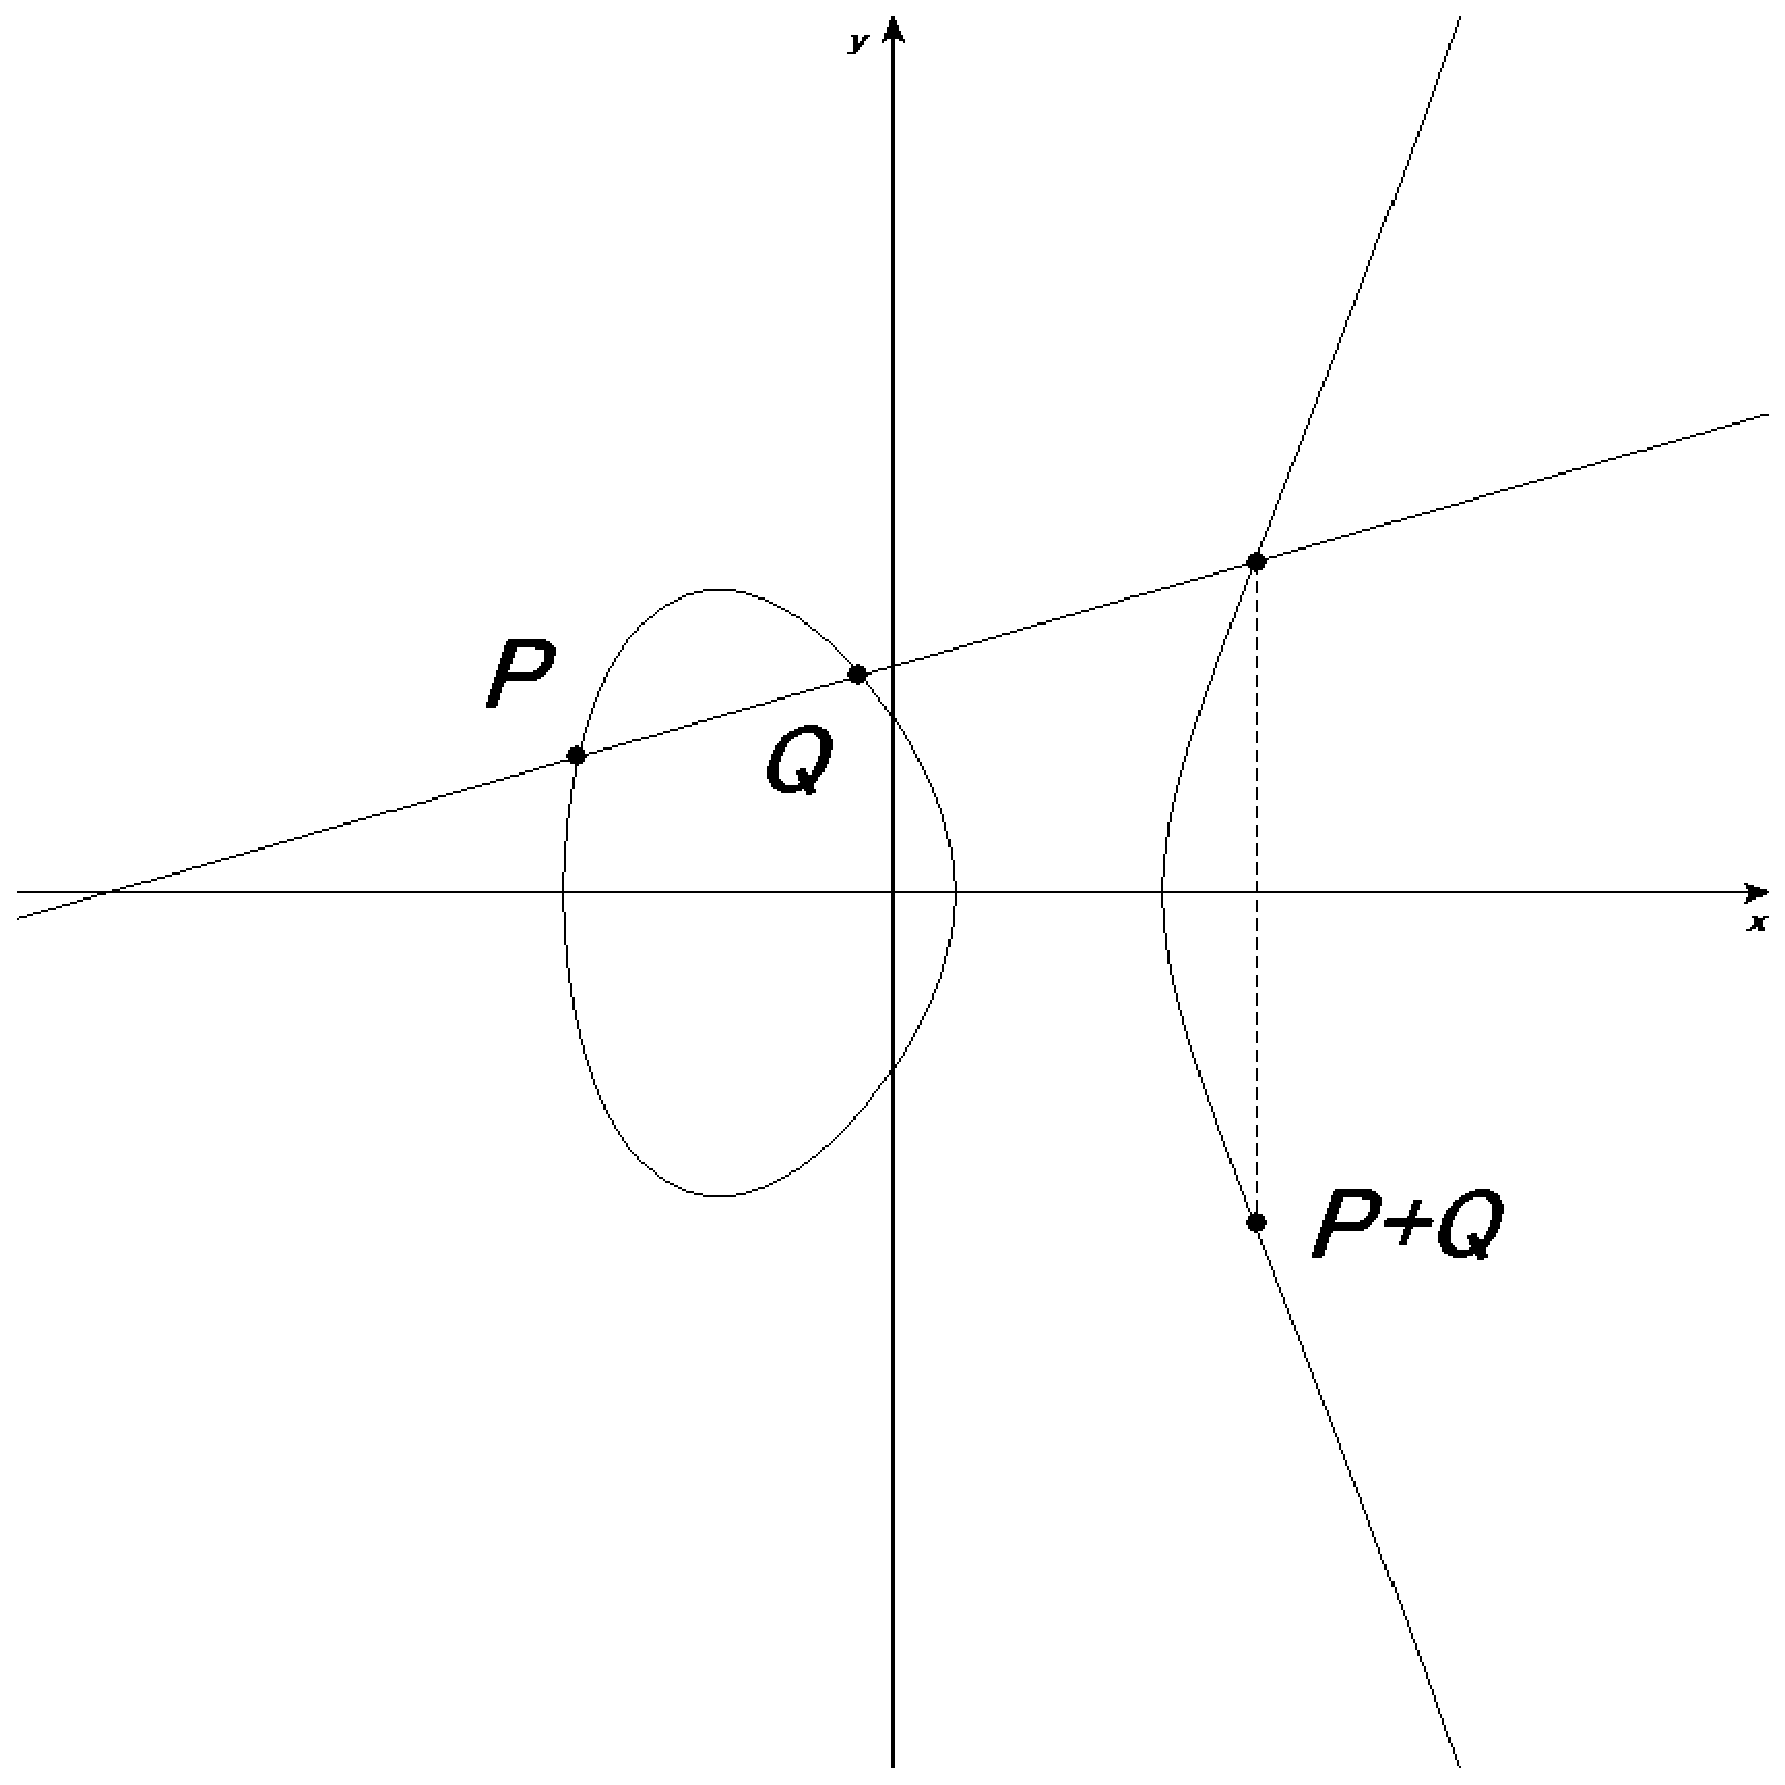
\includegraphics[width=80mm]{elliptic01.eps}
    \end{center}
    \caption{$P+Q$}
    \label{fig:elliptic01.eps}
  \end{minipage}
  \begin{minipage}{0.5\hsize}
    \begin{center}
      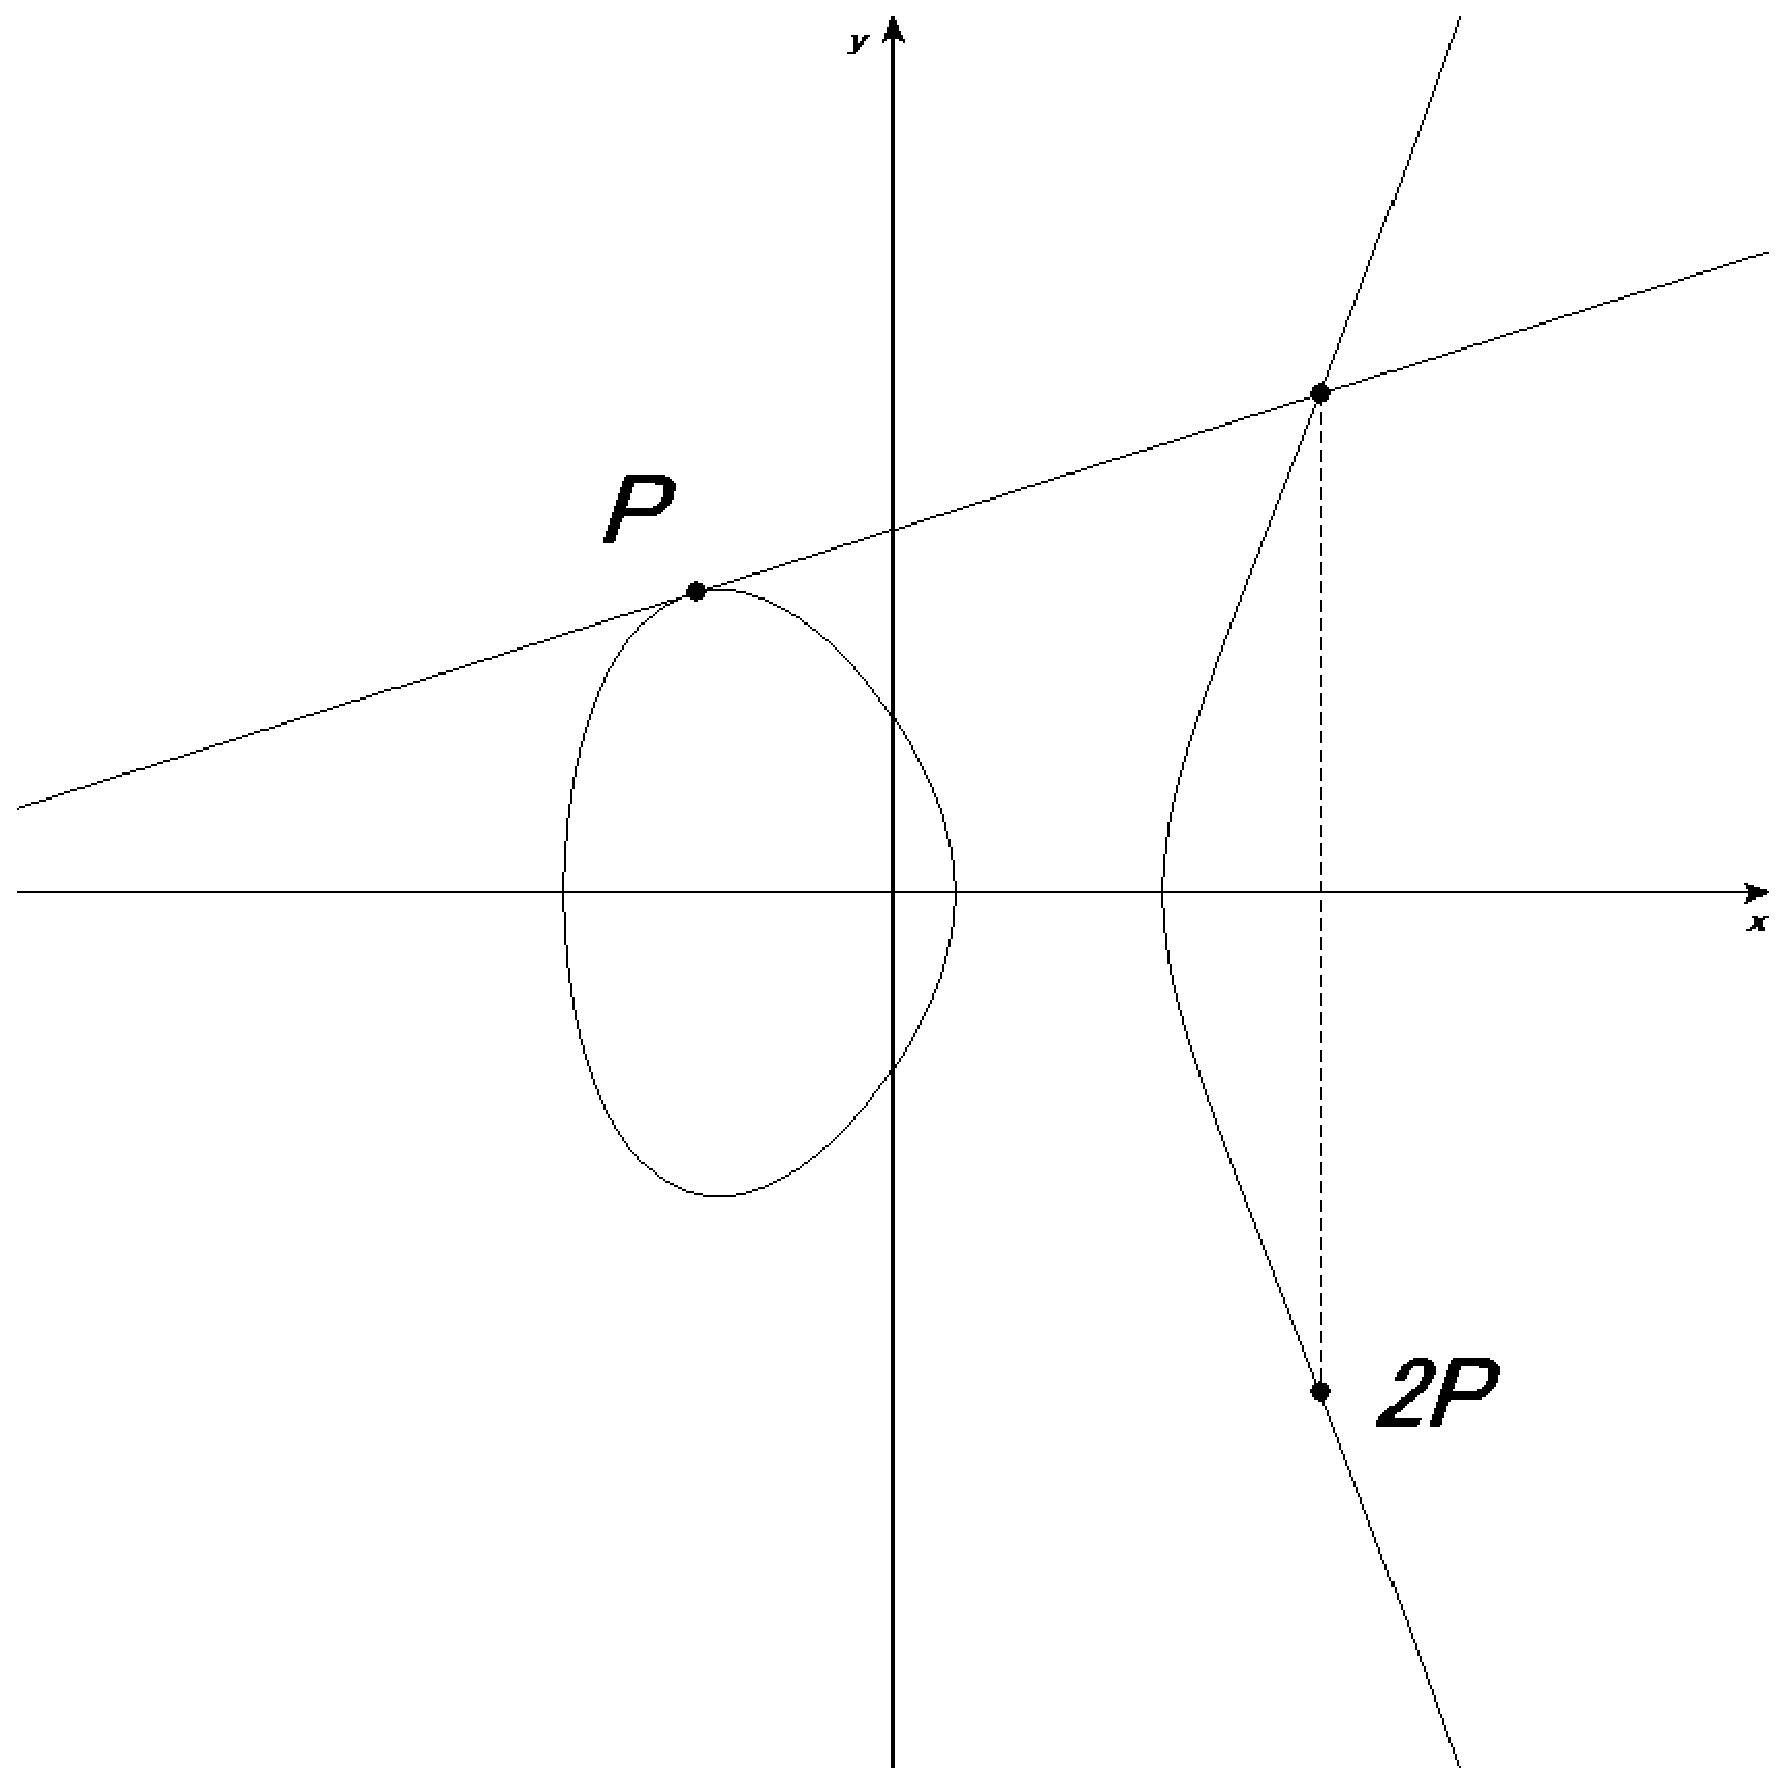
\includegraphics[width=80mm]{elliptic02.eps}
    \end{center}
    \caption{$2P$}
    \label{fig:elliptic02.eps}
  \end{minipage}
\end{figure}
\begin{figure}[htbp]
  \begin{minipage}{0.5\hsize}
    \begin{center}
      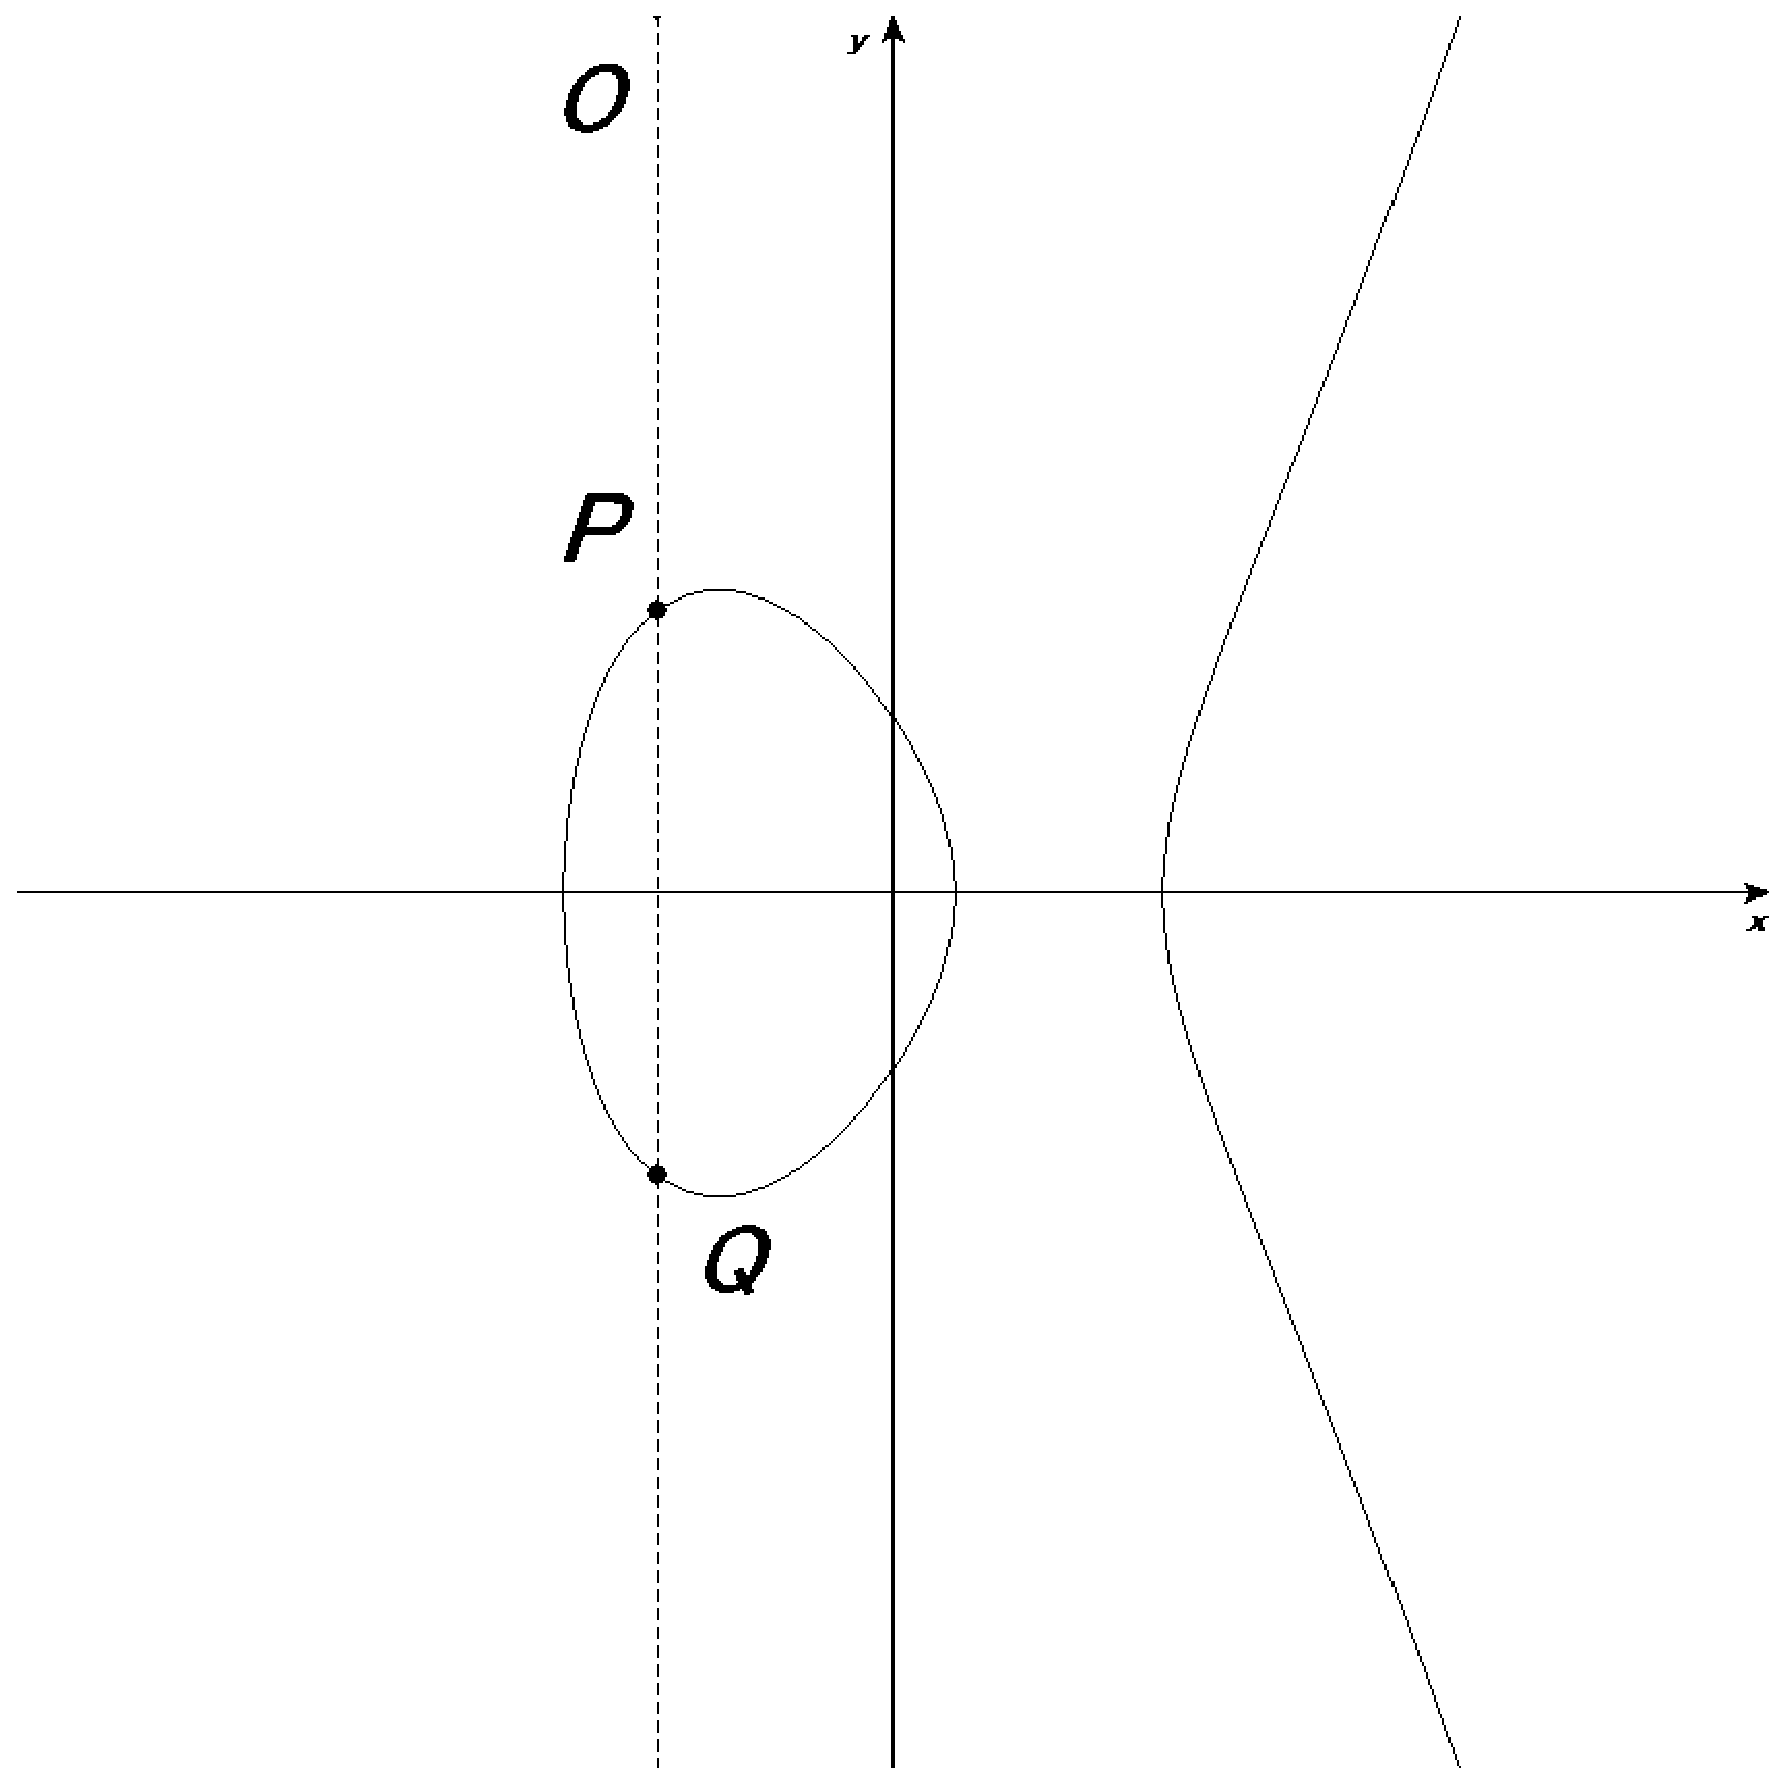
\includegraphics[width=80mm]{elliptic03.eps}
    \end{center}
    \caption{$P+Q=\mathcal{O}$}    \label{fig:elliptic03.eps}
  \end{minipage}
  \begin{minipage}{0.5\hsize}
    \begin{center}
      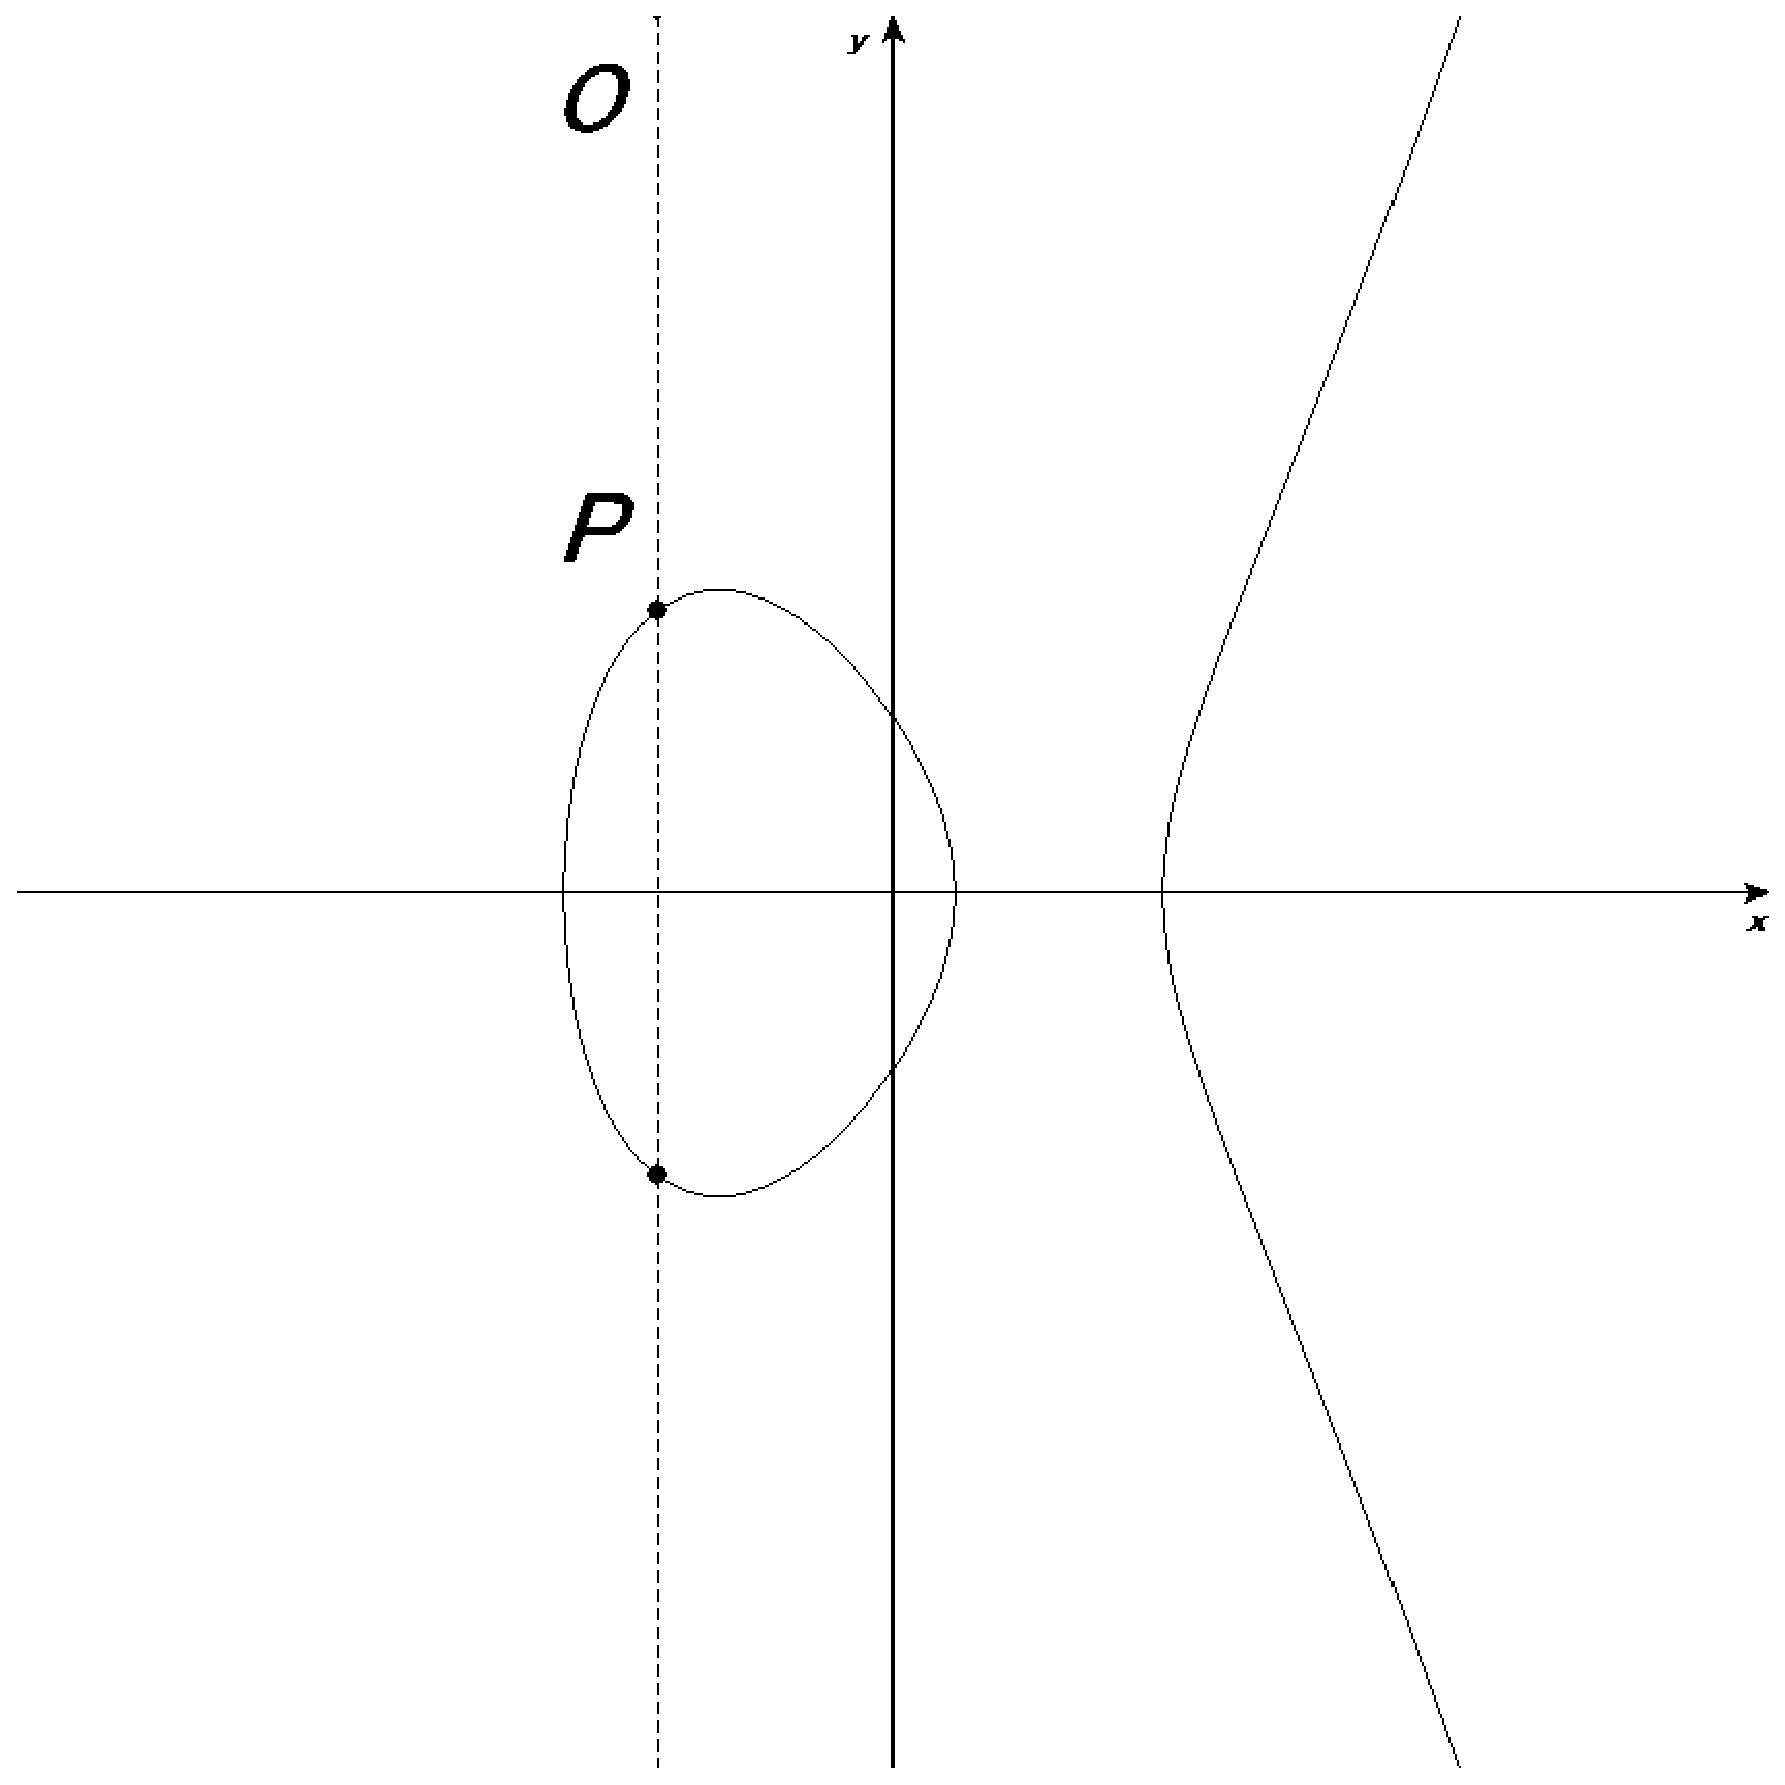
\includegraphics[width=80mm]{elliptic04.eps}
    \end{center}
    \caption{$P+\mathcal{O}=P$}
    \label{fig:elliptic04.eps}
  \end{minipage}
\end{figure}
\par
ここで,$P+Q$を効率的に計算できるよう公式を与える.
楕円曲線を$y^2 = x^3 + ax ^2 + bx +c$とし,各点を
\[
P _1 = (x _1, y _1), \quad P _2 = (x _2, y _2), \quad P*Q = (x _3, y _3), \quad P+Q = (x _3, - y _3)
\]
とする.
このとき,$P _1$と$P _2$を結ぶ直線の方程式は
\[
y = \lambda x + \nu, \quad \lambda = \frac{y _2 - y _1}{x _2 - x _1}, \quad \nu = y _1 - \lambda x _1 
\]
となり,これを楕円曲線の方程式に代入して
\[
x _3 = \lambda ^2 - a - x _1 - x _2, \quad y _3 = \lambda x _3 + \nu
\]
となる.
また,点$P$と点$P$の加算は,2倍算と定義され,$\lambda = \frac{f^{'}(x)}{2y}$を用いて2倍点の$x$座標は
\[
2倍点のx座標 = \frac{x^4 - 2bx^2 - 8cx + b^2 - 4ac}{4x^3 + 4ax^2 + 4bx + 4c}
\]
と表される.\\
\par
\section{楕円離散対数問題}
\subsection{離散対数問題(DLP)}
\par
$p$を素数とし,$g$を$\mathbb{Z}_p^*$の生成元とする.
このとき任意の$y\in \mathbb{Z}_p^*$に対し,
\[
y\equiv g^x\pmod{p}
\]
となる$x$が必ず存在する.
このような$x$を$y$の離散対数という.$y$と$g$が与えられたとき,$y\equiv g^x\pmod{p}$を満たす$x$,
すなわち$x\equiv \log _gy\pmod{p}$を求める問題を離散対数問題という.これは,$y\equiv g^x\pmod{p}$を計算するのは容易だが,$x\equiv \log _gy\pmod{p}$を
求めることは非常に困難であることに基づいている.
\par
\subsection{楕円離散対数問題(ECDLP)}
\par
任意の点$P\in E(\mathbb{F}_q)$に対して,
$\langle P\rangle =\{\mathcal{O},P,2P,3P,\ldots \}$は有限巡回群となる.
この巡回群の位数を$n$
とすると任意の$Q\in \langle P\rangle$に対して,
\[
xP=Q\ \ \ x\in (\mathbb{Z}_n)
\]
となる$x$がただ一つ存在する.
$P$と$Q$が与えられたとき,$x$を求める問題を楕円離散対数問題という.
これは$x$と$P$から$xP=Q$となる$Q$を求めるのは簡単だが,
$P$と$Q$から$x$を求めるのは非常に困難であることに基づいている.\\
\par

\chapter{ペアリング}
%Pairing, divisor, 埋め込み次数の定義, Weil Pairing, Tate Pairing, Miller's Algorithmについて書く. 
\par
\section{ペアリングの定義}
\par
$n$を整数とする.$G_1,G_2$を単位元0の加法アーベル群とする.$G_1,G_2$は位数$n$を持つ.$G_3$は単位元1の乗法に関する位数$n$の巡回群とする.ペアリングというのは以下の関数である.
\[
e:G_1\times G_2\longrightarrow G_3
\]
全てのペアリングは以下の2つの性質を満たす.\\
\begin{description}
\item[\textbf{・双線形性}] 
全ての$P,P' \in G_{1}$と$Q,Q' \in G_{2}$に対して,

e(P+P',Q) = e(P,Q) + e(P',Q),

e(P,Q+Q') = e(P,Q) + e(P,Q')が成り立つ.\\

\item[\textbf{・非退縮性}] \hspace{0em}\\\vspace{-2em}

\item 全ての$P \in G_{1} \ (P \not= 0)$に対して $e(P,Q) \not= 1$となるような$Q \in G_{2}$が存在する.
\item 全ての$Q \in G_{2} \ (P \not= 0)$に対して $e(P,Q) \not= 1$となるような$P \in G_{1}$が存在する.

\end{description}

\par
\section{ペアリングと関係する様々な定義}
\par

\subsection{divisorの定義}
$C$を体$K$上の楕円曲線とし,$C(\overline{K})$を体$K$上の代数閉包上で定義される全ての有理点の集合とする.$C$上のdivisorとは,次のような形式和で表される.
\[
D=\sum\limits_{P\in (C(\overline{K})}n_P(P)
\]
このとき,$n_P\in \mathbb {Z}$は有限であり,$D$は$n_P=0$となるようなものを除いたものとする.$C$上のdivisorの集合はDiv$_{\overline{K}}(C)$
で表され,加法に関して群構造をなす.divisor $D$の台とは,supp$(D) = \langle P \in E|n_P \neq 0 \rangle$であるとする.divisor $D$の次数とはdeg$(D)=\sum\limits_{P}n_P$であるとする. divisor $D$の和とは,sum$(D)=\sum n_PP$であるとする.\\
もし, 直線$f$が$C$上で零でない関数だとすると,点$P$における$f$の重複度ord$_P(f)$を数えることができる.ord$_P(f)$は$f(P)=0$のとき正であり,$f$が点$P$で極ならば負である.また,ord$_P(f)$が1ならば$f=0$と$E$が交差し、2ならば$f=0$が$E$に接し$3P\neq \mathcal{O}$となり,3ならば$f=0$が$E$に接し$3P=\mathcal{O}$となる。零でない関数$f$のdivisorは$(f)$と書き,
\[
\sum\limits_{P\in C(\overline K)}{\rm ord}_P(f)(P)
\]
である.これにより,直線$f,g$のdivisorの計算は$(fg)=(f)+(g)$となり$(f/g)=(f)-(g)$となることがわかる.\\
また,$C$のprincipal divisorとはある関数$f$に対して$(f)$と等しいdivisorのことである.このとき,deg$((f))=0$となる.点$(P,Q)$を通る直線$l_{P,Q}$を考えたとき,この直線のdivisorを求める公式は
\[
{\rm div}(l_{P,Q})=(P)+(Q)+(-(P+Q))-3(\mathcal{O})
\]
で表される.
\par
\subsection{埋め込み次数の定義}
$K _0 = \mathbb{F} _q$を有限体とする.
$E$を$K _0$上で定義された楕円曲線とし,$\# E(K _0)$で割り切られ,$q$と素な整数を$n$とする.
体$K = K _0 (\mu _n)$はある拡大体$\mathbb{F} _{q ^{k}}$とする.
$k$は埋め込み次数や安定乗数と呼ばれ,$(q ^k -1)$が$n$を割り切るようなような最小の正整数である.
$k$というのは,$q$と$n$の関数$k(q, n)$である.
$k$は$n$を法とした$q$の位数なので,$k$は$\phi  _{Eul} (n)$(オイラーの$\phi$関数)で割り切られる.
\par
任意の体$K$と任意の楕円曲線$E$に関して,もし$n$を$\# E(\mathbb{F} _q)$の大きなdivisorとすると,埋め込み次数$k$は大抵の場合とても大きく(bitも$n$と同じ数だけある),そのため体$\mathbb{F} _{q ^k}$上の計算は指数的に複雑になる.\\
\par
\section{Weilの定理}
\par
ある楕円曲線$E/\mathbb {F}_q$に対して,曲線上の有理点の集合$E(\mathbb {F}_q)$を考える.このとき,$E(\mathbb {F}_{q^m})$の位数$\# E(\mathbb {F}_{q^m})$は$E(\mathbb {F}_q)$の位数$\# E(\mathbb {F}_q)$を用いて次のように求められる.
\begin{eqnarray*}
\# E(\mathbb {F}_{q^m})&=&q^m+1-t_{[m]}\\
t_{[m]}&=&\alpha ^m+\beta ^m
\end{eqnarray*}
ただし,$t$を$E(\mathbb {F}_q)$のトレース\ $t=q+1-\# E(\mathbb {F}_q)$とする.このとき,$|t|\le 2 \sqrt{q}$が成り立つ.また,$\alpha ,\beta $は$\alpha \beta =q,\alpha +\beta =t$を満たす複素数である.$t_{[m]}$は$E(\mathbb {F}_{q^m})$のトレースとする.$t_{[m]}$は$E(\mathbb {F}_q)$のトレースを用いて次式で与えられる.
\begin{eqnarray*}
t_{[m]}=\sum\limits _{i=0}^{\left\lfloor m/2\right\rfloor}\frac{m}{m-i} {}_{m-i}C_i(-q)^it^{m-2i}
\end{eqnarray*}ここで,$\left\lfloor m/2\right\rfloor$は$m/2$以下の最大の整数を意味する.Weilの定理を用いることで,定義体を拡大体とした場合の楕円曲線の位数を求めることができ,$\# E(\mathbb {F}_q)$は$\# E(\mathbb {F}_{q^m})$を割り切ることがわかる.\\
\par
\section{Weil ペアリング}
\par
$E$を$K _0$上で定義された楕円曲線とし,$n$を$K _0$の標数と互いに素な整数とする.
$n$で割り切れる位数の$E(\overline{K})$のすべての点の座標で生成された$K _0$の拡大体を$K = K _0(E[n])$で定義する.
Weilペアリングというのは,写像
\[
e _n: E[n] \times E[n] \to \mu _n \subseteq K ^*
\]
で定義される.
$\mu _n$は$\overline{K}$の単位元の$n$乗根とする.
\par
$T \in E[n]$とする.
このとき,${\rm div} (f) = n(T) - n(\mathcal{O})$なる関数$f$が存在する.
$nT' = T$となるような$T' \in E[n ^2]$を選ぶと,${\rm div}(g) = \sigma _{R \in E[n]} ((T' + R) - (R))$
なる関数$g$が存在する.
このとき,点$R \in E[n]$には$n ^2$となる要素が含まれており,その場合は$\sigma (T' + R)$と$\sigma (R)$は
打ち消される.
$g$は$T'$の値によらないので,2つの違う$T'$を取ってきてもそれは$R$による.
よって,${\rm div}(g) = \sigma _{nT'' = T} (T'') - \sigma _{nR = \mathcal{O}} (R)$と表される.
\par
$f \circ n$をある点を$n$倍した後に関数$f$を適応させるような関数とする.
$R \in E[n]$であるような$P = T' + R$を選んだとき,$nP = T$である.
このとき,${\rm div}(f \circ n) = n(\sigma _R (T' + R)) - n(\sigma _R (R)) = {\rm div}(g ^n)$であり,
$f \circ n$は$g ^n$の定数倍である.
適当に$f$を倍算したものを考えれば,$f \circ n = g ^n$である.
$S \in E[n]$とし$P \in E(\overline{K})$とすると,
$g(P + S) ^n = f(n(P + S)) = f(nP) = g(P) ^n$となる.
よって$g(P + S) / g(P) \in \mu _n$となる.
$g(P + S) / g(P)$は$P$と独立となる.
\par
以上より,Weilペアリングというのは,
\[
e _n(S, T) = \frac{g(P + S)}{g(P)}
\]
で定義される.
\par
Weil ペアリングは以下の特性を満たす.
\begin{enumerate}
  \item (双線形性) すべての$P, P', Q, Q' \in E[n]$に対して,
  \[
  e _n(P + P', Q) = e _n(P, Q) e _n(P', Q)
  \]
  かつ
  \[
  e _n(P, Q + Q') = e _n(P, Q) e _n(P, Q')
  \]
  \item (一意性) 全ての$P \in E[n]$に対して,$e(P, P) = 1$
  \item (交換性) 全ての$P, Q \in E[n]$に対して,$e _n(P, Q) = e _n(Q, P) ^{-1}$
  \item (非退化) もし全ての$Q \in E[n]$において$e _n(P, Q) = 1$ならば,$P = \mathcal{O}$
  \item (適合性) もし$P \in E[n m]$かつ$Q \in E[n]$ならば,
  \[
  e _{n m}(P, Q) = e _n([m]P, Q)
  \]
  \item もし$\phi:E \to E'$が2つの$\hat{\phi}$をもつ同種写像であるならば,
  \[
  e _n(\phi(P), Q) = e _n(P, \hat{\phi}(Q))
  \]
\end{enumerate}
\section{Tate ペアリング}
\par
$P \in E(\mathbb{F}_q)[n]$に対してdiv($f_{n, P})=n(P)-n(\mathcal{O})$となる有理関数$f_{n,P} \in E(\mathbb{F}_q)$が存在する. すべての点を$n$倍して得られることなる点の集合を$nE(\mathbb{F}_{q^k})$とすると, その剰余類全体の集合を$E(\mathbb{F}_{q^k})/nE(\mathbb{F}_{q^k})$と表現する. 剰余類の代表元を$Q$として, $D \sim (Q) - (\mathcal{O})$となる因子$D \in \mbox{Div}^0(E)$を選択する. supp(div($f_{n, P})) \cap \mbox{supp} (D) = \not 0$を満足するようにランダムに選んだ点$R \in E(\mathbb{F}_{q^k})$を利用して$D=(Q + R) - (R)とおくと,\ f_{n,P}(D)$を計算可能である. Tate ペアリングは次のように定義可能である. 
\par
\[
\langle \cdot,\cdot\rangle_n:
\left\{
\begin{array}{l}
E(\mathbb{F}_q)[n] \times E(\mathbb{F}_{q^k})/nE(\mathbb{F}_{q^k}) \to \mathbb{F}_{q^k}^\ast /(\mathbb{F}_{q^k}^\ast)^n\\
(P,Q) \mapsto \langle P, Q \rangle _n = f_{n,P}(D)
\end{array}
\right.
\]
\par
Tate ペアリングの値は剰余類全体の集合$\mathbb{F}_{q^k}^\ast/(\mathbb{F}_{q^k}^\ast)^n$に属しており, 一意に定まらない. すなわち, 二つの元$a,\ b \in \mathbb{F}_{q^k}^\ast が元c \in \mathbb{F}_{q^k}を用いてa = bc^n$と表現可能なとき, $a,\ b$は合同となる.ペアリングを利用する方式では$\mathbb{F}_{q^k}^\ast$における一意に定まる値が必要がため, $c^n$を消去する必要がある. $a^{q^k - 1} = 1,\ a \in \mathbb{F}_{q^k}^\ast$の性質を利用して, Tate ペアリングの値に最終べき乗$(q^k - 1) / n$を行うことにより, 一意な値を得ることが可能である. Tate ペアリングの値を最終べき乗したReduced Tate ペアリングを次のように定義する. 
\par
\[
P \in E(\mathbb{F}_q)[n],\ Q \in E(\mathbb{F}_{q^k}),\ \mu_n = \left\{ x \in \mathbb{F}_{q^k}^\ast | x^n = 1 \right\}
\]
とする. \\
\[
\tau \langle P,Q \rangle = \langle P,Q \rangle _n^{(q^k - 1) / n} = f_{n,P}(Q)^{(q^k - 1) / n} \in \mu_n
\]
\par
さらに, Reduced Tate ペアリングの重要な性質として$N = hn$に対して次の式が成立する. 
\par
\[
\tau(P,Q) = \langle P,Q \rangle _n^{(q^k - 1) / n}
\]
\par
これにより, $n$をHamming Weightが小さい$N = hn \in \mathbb{N}$に変更することにより, Miller Algorithmにおけるループ回数は部分群の位数$n$を用いる場合に比べ増加するが, アルゴリズムの総計算量の低減が期待できる. 
Tateペアリングは以下のような性質を持つ.
\begin{enumerate}
  \item (双線形性) 全ての$P, P', Q, Q' \in E[n]$に対して,
  \[
  \langle P + P', Q \rangle _n = \langle P, Q \rangle _n \langle P', Q \rangle _n
  \]
  かつ
  \[
  \langle P, Q + Q' \rangle _n = \langle P, Q \rangle _n \langle P, Q' \rangle _n
  \]
  \item (非退化) $\mathbb{F}_{q^k}$を有限体とする.全ての$P \in E(\mathbb{F}_{q^k})[n] \ (P \not= 0)$に対して,
  $\langle P, Q\rangle _n \not= 1$となるような$Q \in E(\mathbb{F}_{q^k}) / nE(\mathbb{F}_{q^k})$が存在する.
  同様にして,全ての$Q \in E(\mathbb{F}_{q^k}) / nE(\mathbb{F}_{q^k}) \ (Q \notin nE(\mathbb{F}_{q^k}))$に対して,
  $\langle P, Q\rangle _n \not= 1$となるような$P \in E(\mathbb{F}_{q^k})[n]$が存在する.
  \item (ガロアの不変性) もし$\sigma \in \rm{Gal}\it{(\overline{\mathbb{F}}_{q^k} / \mathbb{F}_q)}$とすると,
  $\langle \sigma (P), \sigma (Q) \rangle _n = \sigma(\langle P, Q \rangle _n)$
  である.
\end{enumerate}

\par
\section{Miller Algorithm}
\par
Miller Algorithm\cite{MIA}とは,Weilペアリングを多項式時間で求めるアルゴリズムである.
また,Miller AlgorithmはTateペアリングの計算にも用いることができる.TateペアリングにおいてMiller Algorithmを考える.定義式
\[
f_P(D_Q)^{{(q^k-1)}/n}
\]
から,以下の条件を満たす有理関数$f_P$の計算に帰着される.
\[
{\rm div}(f_P)=n(P)-n(\mathcal{O})
\]
ここで$f_h$を
\[
{\rm div}(f_h)=h(P)-(hP)-(h-1)(\mathcal{O})
\]
を満たす有理関数とする.点$iP$と$jP$を通る直線を$l_{iP,jP}$とし,点$(i+j)P$を通る垂線を$v_{(i+j)P}$とすると,Miller Algorithm中で再帰的に$f_P=f_h$を求めるための基本公式
\[
{\rm div}(f_{i+j})-{\rm div}(f_i)-{\rm div}(f_j)={\rm div}\Bigl(\frac{l_{iP,jP}}{v_{(i+j)P}}\Bigr)
\]
は次のように証明される.
\begin{proof}
直線のdivisorの公式
\[
{\rm div}(l_{P,Q})=(P)+(Q)+(-(P+Q))-3(\mathcal{O})
\]
より,
\begin{eqnarray*}
{\rm div}\Bigl(\frac{l_{iP,jP}}{v_{(i+j)P}}\Bigr)&=&{\rm div}(l_{iP,jP})-{\rm div}(v_{(i+j)P})\\
&=&\left\{(iP)+(jP)+(-(i+j)P)-3(\mathcal{O})\right\}-\left\{((i+j)P)+(-(i+j)P)-2(\mathcal{O})\right\}\\
&=&(iP)+(jP)-((i+j)P)-(\mathcal{O})
\end{eqnarray*}となる.一方$f_h$の定義から
\begin{eqnarray*}
{\rm div}(f_{i+j})-{\rm div}(f_i)-{\rm div}(f_j)&=&\left\{(i+j)P-((i+j)P)-(i+j-1)(\mathcal{O})\right\}\\
&\ \ \ &-\left\{i(P)-(iP)-(i-1)(\mathcal{O})\right\}-\left\{j(P)-(jP)-(j-1)(\mathcal{O})\right\}\\
&=&(iP)+(jP)-((i+j)P)-(\mathcal{O})
\end{eqnarray*}が得られ,両者は等しくなる.\\
従って
\[
{\rm div}(f_{i+j})={\rm div}(f_i)+{\rm div}(f_j)+{\rm div}\Bigl(\frac{l_{iP,jP}}{v_{(i+j)P}}\Bigr)={\rm div}\Bigl(f_if_j\frac{l_{iP,jP}}{v_{(i+j)P}}\Bigr)
\]
これより,再帰的公式
\[
f_{i+j}=\Bigl(f_if_j\frac{l_{iP,jP}}{v_{(i+j)P}}\Bigr)
\]が得られた.
\end{proof}
これを用いてMiller Algorithmは,$(f) = n(P) - n(\mathcal{O})$となるような関数$f$を構成している.次にMiller Algorithmを示す. 
\par
\begin{table}[htbp]
 \begin{center}
  \begin{tabular}{|l|}
     \hline
     Input: $n, \ P \in E(\mathbb{F}_q)[n], \ Q \in E(\mathbb{F}_{q^k})$ \\
     Output: $f \in \mathbb{F}_{q^k}$  \\
     \hline
     1: \quad $Q' \in _R E(\mathbb{F}_{q^k})$\\
     2: \quad $S=Q+Q' \in E(\mathbb{F}_{q^k})$\\
     3: \quad $V \gets P, \ f \gets 1$\\
     4: \quad $n=\sum^{l-1}_{i=0} n_i 2^i, \ n_i \in {0,1}$\\
     5: \quad for $j \gets l-1$ down do 0\\
     6: \quad \quad $f \gets f^2 \cdot \frac{g_{V,V}(S)g_{2V}(Q')}{g_{2V}(S)g_{V,V}(Q')}$\\
     7: \quad \quad $V \gets 2V$\\
     8: \quad if $n_j = 1$ then\\
     9: \quad \quad $f \gets f \cdot \frac{g_{V,P}(S)g_{V+P}(Q')}{g_{V+P}(S)g_{V,P}(Q')}$\\
     10: \quad \quad $V \gets V+P$\\
     11: \quad return $f$\\
     \hline
   \end{tabular}
 \end{center}
 \caption{Miller Algorithm}
\end{table}
\par
Miller Algorithmの主な反復は$\log _2(n)$の繰り返しなので,二重の操作は$\log _2(n)$時間で成し遂げられる.
5行目から10行目までの掛け算と足し算の演算は$n$のHamming Weight以下で計算される.
それゆえMiller Algorithmは多項式時間で動作する.
\par
適当な点$S$を選ぶ1つの方法としては,$E(\mathbb{F}_{q^k})$上の点をランダムに選ぶことである.
$n$が大きいとき,このアルゴリズムは$S = [i]P$を取ることによって容易に決定的になる.
このとき,$i$の2進展開は$n$の2進展開の一部ではないとする($P \in E(\mathbb{F} _q)$かつ$Q \in E(\mathbb{F} _q)$ならば$S = Q$を取る).
\par
このアルゴリズムの変化量は,直線プログラムとして関数$f$に対して明確な表示で出力される(例えば,もしそれが因数分解された形式を保つならば,小さな多項式の累乗の積として多項式の保存を必要とする).\\

\par
\section{distortion map}
\par

distortion mapというのは,$E(\mathbb{F} _q)$上の点を$E(\mathbb{F} _{q ^k})$上の点に写像するような
非線形な自己順同型写像である.
点$P \in E(\mathbb{F} _q)$が位数$n$の点を持つとし,$k > 1$とする.
$E(\mathbb{F} _{q ^k})$は位数$n ^2$の点を持たないとすると,$E$上の準同型$\psi$によって
$\psi(P) \notin E(\mathbb{F} _{q ^k})$ならば$e(P, \psi(P)) \not= 1$となる.
\par
ペアリングの非退化について,distortion mapが用いられる場合,$E$の非線形自己準同型$\psi$を用いて,
$\hat{e} : G _1 \times G _1 \to G _3$を
\[
\hat{e}(P, Q) = \hat{e}(P, \psi(Q))
\]
と定義することにより,非退化において全ての$P \in G _1$において
\[
\hat{e}(P, P) = \hat{e}(P, \psi(P)) \not= 1
\]
である.
これは暗号方式を用いる際にかなり重要である.
一意的な値を得るためには,ペアリングの値が$1$とならない場合についてのみ考えなければいけないからである.\\
\par
\section{Supersingular curve}
\par
上記のdistortion mapを持つような$\mathbb{F} _q$上の楕円曲線$E$はsupersingularとなる.
Supersingularとは,以下の条件を1つでも満たす場合をいう.
\begin{enumerate}
  \item $\# E(\mathbb{F} _q) \equiv 1 \ (\bmod p)$ 
        ($p \mid t$で$\# E(\mathbb{F} _q) = q + 1 - t$と等価)
  \item $E$が$\overline{\mathbb{F}} _q$上で位数$p$の点を取らない.
  \item $\overline{\mathbb{F}} _q$上の$E$の準同型環が非可換である.
\end{enumerate}
もし$E$がsupersingularでない場合,ordinaryであるという.
Supersingular curveは限られており,それは埋め込み次数が$6$以下であるので,
ペアリングを用いた暗号系に適している.\\
\chapter{ペアリング演算の高速化}
%Miller Algorithmの発展, BKLS,window Algorithmについて書く.
\section{Signed Miller Algorithm}
第4章で述べたMiller Algorithmでは部分群の位数$n$を2進展開していた. Signed Miller Algorithmは符号付き2進展開を用いる手法である. 次にそのアルゴリズムを示す.
\par
\begin{table}[htbp]
 \begin{center}
  \begin{tabular}{|l|}
     \hline
     Input: $n, \ P = (x_P,y_P) \in E(\mathbb{F}_q)[n], \ Q = (x_Q,y_Q) \in E(\mathbb{F}_{q^k})$ \\
     Output: $f \in \mathbb{F}_{q^k}$  \\
     \hline
     1: \quad $Q' \in _R E(\mathbb{F}_{q^k})$\\
     2: \quad $S=Q+Q' \in E(\mathbb{F}_{q^k})$\\
     3: \quad $V \gets P, \ f \gets 1,\ f_{-1} = \frac{1}{x_Q - x_P}$\\
     4: \quad $n=\sum^{l - 1}_{i=0} n_i 2^i, \ n_i \in \{-1,0,1\},\ n_0 = 1$\\
     5: \quad for $j \gets l - 1$ down do 0\\
     6: \quad \quad $f \gets f^2 \cdot \frac{g_{V,V}(S)g_{2V}(Q')}{g_{2V}(S)g_{V,V}(Q')}$\\
     7: \quad \quad $V \gets 2V$\\
     8: \quad if $n_j = 1$ then\\
     9: \quad \quad $f \gets f \cdot \frac{g_{V,P}(S)g_{V + P}(Q')}{g_{V + P}(S)g_{V,P}(Q')}$\\
     10: \quad \quad $V \gets V + P$\\
     11: \quad if $n_j = -1$ then\\
     12: \quad \quad $f \gets f \cdot f_{-1} \cdot \frac{g_{V,P}(S)g_{V - P}(Q')}{g_{V - P}(S)g_{V,P}(Q')}$\\
     13: \quad \quad $V \gets V - P$\\
     14: \quad return $f$\\
     \hline
   \end{tabular}
 \end{center}
 \caption{Signed Miller Algorithm}
\end{table}
このように符号付きで展開する方法は後述のアルゴリズムでも同様に用いることができる.
\clearpage
\section{高速化手法}
supersingular curveにおけるReduced Tate ペアリングの高速化手法がBarretoらによっていくつか提案された\cite{BKLS01}. それを次に列挙する.
\subsection{部分体の要素による乗算}
埋め込み次数$k$の因子を$d$とすると, ペアリングの値を変えずに非零な要素$x \in {F}_{q^d}をf_{n,P}(Q)$に乗じることが可能である. $q^k - 1 = (q^d - 1)\sum^{k / d - 1}_{i = 0} q^{id}$と因数分解化のであり, $k > 1のときn | q^k -  1,\ n \not | q^d - 1$となるため, $n | \sum^{k / d - 1}_{i = 0} q^{id}$である. すなわち, $(q^k - 1) / n は因子としてq^d - 1$を必ず含んでいる. よって, $f_{n,P}(Q)は最終べき乗(q^k - 1) / n$の処理を行うことにより, フェルマーの小定理より乗じた値$x^{(q^k - 1) / n} = 1$となる.
\subsection{点による因子の置換}
ペアリングの値は, 引数として与える$Q \in E(K)$とランダムに選択される$R \in E(K)$から構成される因子$D = (Q + R) - (R)$を用いて計算されるが, 因子$Dを点Q$と置換しても正しく計算可能で$P \in E(K_0)[n],\ Q \in E(K)$は線形独立な点とするとき, 次の式が成立する.
\par
\[
e(P,Q) = f_{n,P}(Q)^{q^k-1}
\]
\subsection{分母消去}
Supersingular Curveであれば, $Q'_1 \in E(K_0)$にdistortion mapを適用させることにより, $Q_1 = \psi (Q'_1) \in E(K)$を得る. Ordinary Curveであれば, twist $E'$上の点$Q'_2 \in E(\mathbb{F}_{q^e})からQ'_2 = \psi (Q'_2) \in E(K)を得る$. ここで, $m = \mbox{gcd}(k,d),\ e = k/m$である. よって$Q = (x,y) \in E(K)においてx \in \mathbb{F}_{q^{k/2}} となるとき$, Miller Algorithmの2倍算または加算ステップに出現する分母の要素$g_{2V},g_{V + P}はe(P,Q)$の値を変更することなく省略可能である.
\subsection{群位数のHamming Weight}
Miller Algorithmは部分群の位数$n$に対する2進展開法に基づき, ペアリングの値を計算しているため, 加算ステップの処理回数は$n$のHamming Weight(2進展開した値における1の総数)に依存する. ランダムに選択された$n$の平均的なHamming Weightはビット長の半分程度になるが, 部分群の位数として$n = 2^\alpha \pm 2^\beta \pm 1$を選択することにより, ペアリング演算コストを大幅に抑えることが可能である.
\subsection{最終べき乗の高速化}
Pairing-friendly field $K$における最終べき乗$(q^k - 1) / n$を想定する. $k$次の円分多項式 $\Phi _k(p)$とすれば, $n|q^k - 1$であるため, 次のように変形できる.
\[
f^{(q^k - 1) / n} = (f^{(q^k - 1) / \Phi _k(q)})^{(\Phi _k(q) / n)}
\]
最終べき乗のコストは$(\Phi _k(q) / n)$乗のコストと同等, $(\Phi _k(q) / n)$のビット長は$(\Phi _k(q) / k)\mbox{log} _2 (q^k) - \mbox{log} _2 (n)$となる.
\clearpage
\section{BKLS Algorithm}
前述した高速化手法を用いて, supersingular curveのdistortion map $\psi$ を利用して分母消去の手法を適用したBKLS Algorithm \cite{BKLS02}を次に示す. ordinary curveの場合, $Q' \in E'(K)$として, distortion mapではなくtwistの同型写像 $\psi _d$を用いる.
\vspace{0.5cm}
\par
\begin{table}[htbp]
 \begin{center}
  \begin{tabular}{|l|}
     \hline
     Input: $P,\ Q \in E(K_0)[n]$\\
     Output: $f \in K$\\
     \hline
     1: \quad $f \gets 1,\ V \gets P$\\
     2: \quad $n=\sum_{l-1}^{i=0} n_i 2^i, \ n_i \in \{0,1\}$\\
     3: \quad for $j \gets l-1$ down 0 do 0\\
     4: \quad \quad $f \gets f^2 \cdot g_{V,\ V}(\psi (Q))$\\
     5: \quad \quad $V \gets 2V$\\
     6: \quad if $n_j = 1$ then\\
     7: \quad \quad $f \gets f \cdot g_{V,\ P}(\psi (Q))$\\
     8: \quad \quad $V \gets V+P$\\
     9: \quad return $f$\\
     \hline
   \end{tabular}
 \end{center}
 \caption{BKLS Algorithm}
\end{table}
\vspace{-0.5cm}
\par

\section{Window Miller Algorithm}
window Miller アルゴリズムは、オンライン事前演算 を用いる方法である\cite{WML}。

まず、$i=1,\ldots,2w-1$ に対して2$w$ 個の楕円曲線上の点 $P_i = iP$ を求め、各 $P_i$ において
$i(P) − i(O) = (P _i) − (O) + div(f _i)$ が成り立つような有理式 $f _i$ に対し、
$f' _i  = f' _i(Q + S) /f _i(S)$ となる $f' _i ∈ \mathbb{F}_{q^k}$ を求める。
この $P_i, f' _i$ を用いることで、楕円加算および直線 $g _{P, -P_i}$, 垂線 $g _{P_i , \mathcal{O}}$
に関係する演算を削減する。上記アルゴリズムの説明では、簡単にするために $w|l$ を仮定している。
 Miller のアルゴリズムでは n のハミング重み $wH (n)$ 回の楕円加算を行っていたが、window Millerアルゴリズムでは、$l/w$ 回行うことになるため、適切な$w$を用いれば、楕円加算および直線 $g _{P, -P_i}$, 垂線 $g _{P_i, \mathcal{O}}$ の計算を削減することができる。
\par

\begin{table}[htbp]
 \begin{center}
  \begin{tabular}{|l|}
     \hline
     Input: $n, \ P \in E(\mathbb{F}_q)[n], \ Q \in E(\mathbb{F}_{q^k}) \ S \in E(\mathbb{F}_{q^k})$ \\
     Output: $f \in \mathbb{F}_{q^k}$  \\
     \hline
     (online computation) \\
     1: \quad $P_1 = P, f'_1=1 $\\
     2: \quad for $i \gets 2$ up to do $2^w -1$\\
     3: \quad \quad $P_i \gets P + P_{i-1} $\\
     4: \quad \quad $f'_i \gets f'_{i-1} \cdot \frac{g_{P,-P_i}(S)g_{\mathcal{O},P_i}(Q+S)}{g_{P,-P_i}(S)g_{\mathcal{O},P_i}(Q+S)}$\\
     (main computation) \\
     5: \quad $V \gets P, f \gets 1 $\\
     6: \quad $n=\sum^{l - 1}_{i=0} n_i 2^i, \ n_i \in \{0,1\},\ n_0 = 1$\\
     7: \quad for $ n-1 \gets i$ down to 0 step w\\
     8: \quad step 8-1 から 8-2 をw回繰り返す\\
     8-1: \quad\quad $V \gets 2V $\\
     8-2: \quad \quad $f \gets f^2 \cdot \frac{g_{V,-2V}(Q+S)g_{\mathcal{O},2V}(S)}{g_{V,-2V}(Q+S)g_{\mathcal{O},2V}(S)}$\\

     9: \quad $n' \gets =\sum^{j=i-w+1}_{i} n_{j}2^{j-i+w-1} $\\
     10: \quad if $n' \neq 0$ then\\
     10-1: \quad \quad $f \gets ff'_m \cdot \frac{g_{V,P_m}(Q+S)g_{\mathcal{O},V+P_m}(S)}{g_{V,P_m}(Q+S)g_{\mathcal{O},V+P_m}(S)}$ \\
     10-2: \quad \quad $V \gets V + P_{n'} $\\
     11: \quad return $f$\\
     \hline
   \end{tabular}
 \end{center}
 \caption{Window Miller Algorithm}
\end{table}

\chapter{既存研究と提案手法}
%既存手法であるwindow法, NAF, left-to-right, double-base chains(k=4, 6, 8)について書く.\\
%提案手法であるdouble-base chains(k=2)について, 実装法などを書く.
\section{提案手法のアルゴリズム}
BKLS Algorithm, Window Miller Algorithmを組みわせることで新しい高速化手法を提案する。以下にそのアルゴリズムを示す.
\par
\begin{table}[htbp]
 \begin{center}
  \begin{tabular}{|l|}
     \hline
     Input: $n, \ P, Q \in E(\mathbb{F}_q)[n]$ \\
     Output: $f \in \mathbb{F}_{q^k}$  \\
     \hline
     (online computation) \\
     1: \quad $P_1 = P, f'_1=1 $\\
     2: \quad for $i \gets 2$ up to do $2^w -1$\\
     3: \quad \quad $P_i \gets P + P_{i-1} $\\
     4: \quad \quad $f'_i \gets f'_{i-1} \cdot g_{P_i,\ P}(\psi (Q))$\\

     (main computation) \\
     5: \quad $V \gets P, f \gets 1 $\\
     6: \quad $n=\sum^{l - 1}_{i=0} n_i 2^i, \ n_i \in \{0,1\},\ n_0 = 1$\\

     7: \quad for $ n-1 \gets i$ down to 0 step w\\
     8: \quad step 8-1 から 8-2 をw回繰り返す\\
     8-1: \quad \quad $V \gets 2V $\\
     8-2: \quad \quad $f \gets f^2 \cdot g_{V,\ V}(\psi (Q))$\\

     9: \quad $m' \gets =\sum^{j=i-w+1}_{i} m[j]2^{j-i+w-1} $\\
     10: \quad if $m' \neq 0$ then\\
     10-1: \quad \quad $f \gets ff'_m \cdot g_{V,\ P_m}(\psi (Q))$ \\
     10-2: \quad \quad $V \gets V + P_{m'} $\\
     11: \quad return $f$\\
     \hline
  \end{tabular}
 \end{center}
 \caption{Window方を用いたBKLS Algorithm}
\end{table}
\par
\clearpage

\section{提案手法の計算量}
Miller Algorithm, BKLS Algorithm, Window Miller Algorithm, 提案手法のアルゴリズムの計算量を比較する。
\par
Millerのアルゴリズムにおける演算部分のステップを加算(TADD), 2倍算(TDBL)に分ける. \cite{TATE}によると、それぞれの計算コストは次のようになっている.
\begin{table}[htbp]
 \begin{center}
  \begin{tabular}{|l|c|}
  \hline
  演算 & 計算コスト \\
  \hline
  TADD & $4M_k + (6k+10)M + 4S$ \\
  \hline
  TDBL & $4M_k + 2S_k + (6k+7)M + 7S$ \\
  \hline
  \end{tabular}
 \end{center}
 \caption{各演算の計算コスト}
\end{table}
\par
ただし、$F_q$ 上の乗算、自乗の演算量を $M$, $S$, $F_{q^k}$ 上の乗算、自乗の演算量を $M_k$, $S_k$ であらわしている。$k$ が比較的小さい値 (supersingular な楕円曲線の場合、$k = 2, 3, 6$) であることを考えると、ほぼ $Mk = k^2M$ と考えられる。ここで、 $S = M$ とすると \\

\begin{table}[htbp]
\begin{center}
\begin{tabular}{|l|c|}
\hline
 演算 & 計算コスト\\
 \hline
 TADD & $(4k^2 + 6k + 14)M$ \\
 \hline
 TDBL & $(6k^2 + 6k + 14)M$ \\
 \hline
\end{tabular}
\end{center}
\caption{計算量(近似)}
\end{table}

$n$を$l$ビットのランダムな数とし,これらを用いて Miller Algorithm, BKLS Algorithm, Window Miller Algorithm, 提案手法のアルゴリズムの計算量は次のように表される.
\begin{table}[htbp]
 \begin{center}
  \begin{tabular}{|l|c|c|c|}
  \hline
  Algorithm & 計算コスト \\
  \hline
  Miller Algorihtm & l \times TDBL+ (l/2)TADD \\
  \hline
  Window Miller Algorithm & l \times TDBL+ (n/w +2^w-2)TADD \\
  \hline
  BKLS Algorithm & l \times TDBL+ (l/2)TADD  \\
  \hline
  提案手法 & l \times TDBL+ (n/w +2^w-2)TADD \\
  \hline
  \end{tabular}
 \end{center}
 \caption{各手法の計算コスト}
\end{table}

\par

例として, $k=6$,$n=170$, $w=4$の場合を考えると

\begin{table}[htbp]
 \begin{center}
  \begin{tabular}{|l|c|c|c|}
  \hline
  Algorithm & 計算コスト \\
  \hline
  Miller Algorihtm & 55590M \\
  \hline
  Window Miller Algorithm & 48009M \\
  \hline
  BKLS Algorithm &   \\
  \hline
  提案手法 &  \\
  \hline
  \end{tabular}
 \end{center}
 \caption{各手法の計算コスト}
\end{table}


\chapter{実行結果}
\section{実行結果}
\subsection{実装環境}
\noindent プロセッサ: Intel(R) Xeon(TM) CPU 3.40GHz\\
メモリ: 2046MB RAM\\
OS: Microsoft Windows XP Professional\\
プログラミング言語: Magma ver.2.14-6

\subsection{実装条件}
\noindent
部分群の位数$n$はランダムに選ぶ. \\
計測は演算部分だけに対して1000回行い, その平均を取った. \\
楕円曲線は埋め込み次数$k=2,\ 4,\ 6$でordinary curveを使用した. \\
実験で使用した曲線は以下の通り. $k=4$の曲線は\cite{OPM}, $k=6$の曲線は\cite{GMM}の例題から引用した. 
\begin{enumerate}
\item $k=2のとき,\ y^2=x^3+x$\\
\item $k=4のときy^2 = x^3 - 3x + b,\ b=2993400528565252484131025435851646783754072514402$\\
\item $k=6のときy^2 = x^3 - 3x + b,\ b=1067782606939229981648974648369145174879546988730$\\
\end{enumerate}
\clearpage
\subsection{実行結果}
$\mbox{log}n \approx 80,120,160$のときの従来手法と提案手法の計算コストと計算時間を次の表に示す. \\
%\vspace{7mm}
\begin{table}[htb]
 \begin{center}
  \begin{tabular}{|l|c|c|}
  \hline
  82bit($b_{max} = 50,\ t_{max} = 20,\ m = 13$) & 計算コスト& 計算時間\\
  \hline
  Miller Algorithm & 3329 & 12.9ms \\
  \hline
  Signed Miller Algorithm & 2906 & 11.3ms \\
  \hline
  Double-Base Chainsを用いたMiller Algorithm & 2487 & 9.6ms \\
  \hline
  \end{tabular}
 \end{center}
 \caption{$k=2,\ \mbox{log}n \approx 80$}
\end{table}
\begin{table}[htb]
 \begin{center}
  \begin{tabular}{|l|c|c|}
  \hline
  120bit($b_{max} = 68,\ t_{max} = 33,\ m = 13$) & 計算コスト& 計算時間\\
  \hline
  Miller Algorithm & 4885 & 21.1ms \\
  \hline
  Signed Miller Algorithm & 4242 & 18.6ms \\
  \hline
  Double-Base Chainsを用いたMiller Algorithm & 3483 & 15.5ms \\
  \hline
  \end{tabular}
 \end{center}
 \caption{$k=2,\ \mbox{log}n \approx 120$}
\end{table}
\begin{table}[htb]
 \begin{center}
  \begin{tabular}{|l|c|c|}
  \hline
  159bit($b_{max} = 97,\ t_{max} = 39,\ m = 17$) & 計算コスト& 計算時間\\
  \hline
  Miller Algorithm & 6481 & 32.9ms \\
  \hline
  Signed Miller Algorithm & 5614 & 29.2ms \\
  \hline
  Double-Base Chainsを用いたMiller Algorithm & 4565 & 25.1ms \\
  \hline
  \end{tabular}
 \end{center}
 \caption{$k=2,\ \mbox{log}n \approx 160$}
\end{table}
\begin{table}[htb]
 \begin{center}
  \begin{tabular}{|l|c|c|}
  \hline
  161bit($b_{max} = 72,\ t_{max} = 56,\ m = 24$) & 計算コスト& 計算時間\\
  \hline
  Miller Algorithm & 6563 & 43.8ms \\
  \hline
  Signed Miller Algorithm & 5684 & 42.5ms \\
  \hline
  Double-Base Chainsを用いたMiller Algorithm & 4697 & 34.9ms \\
  \hline
  \end{tabular}
 \end{center}
 \caption{$k=2,\ \mbox{log}n \approx 160$}
\end{table}
\begin{table}[htb]
 \begin{center}
  \begin{tabular}{|l|c|c|}
  \hline
  162bit($b_{max} = 113,\ t_{max} = 31,\ m = 45$) & 計算コスト& 計算時間\\
  \hline
  Miller Algorithm & 12623 & 66.2ms \\
  \hline
  Signed Miller Algorithm & 9273 & 64.0ms \\
  \hline
  Double-Base Chainsを用いたMiller Algorithm & 8796 & 59.0ms \\
  \hline
  \end{tabular}
 \end{center}
 \caption{$k=4,\ \mbox{log}n \approx 160$}
\end{table}
\begin{table}[htbp]
 \begin{center}
  \begin{tabular}{|l|c|c|}
  \hline
  159bit($b_{max} = 80,\ t_{max} = 49,\ m = 36$) & 計算コスト& 計算時間\\
  \hline
  Miller Algorithm & 19795 & 78.4ms \\
  \hline
  Signed Miller Algorithm & 13289 & 77.8ms \\
  \hline
  Double-Base Chainsを用いたMiller Algorithm & 12205 & 64.8ms \\
  \hline
  \end{tabular}
 \end{center}
 \caption{$k=6,\ \mbox{log}n \approx 160$}
\end{table}
\vspace{2cm}
\par
提案手法は従来手法に比べて表7.1から82bitでは34\%, 18\%, 表7.2から120bitでは36\%, 20\%, 表7.3から159bitでは31\%, 16\%, 表7.4から161bitでは25\%, 22\%の高速化を実現した. 
さらに既存研究を実装した結果、表7.5から$k=4$で160bitのとき,  12\%, 8\%, 表7.6から$k=6$で160bitのとき, 21\%, 20\%の高速化を実現した. 
\clearpage
\chapter{考察と今後の課題}
\section{考察}
実行結果の表を二つに分類して考察する.\\

\noindent (1) 表7.1, 7.2, 7.3について考える. \\
\par
計算コストからMiller Algorithm, Signed Miller Algorithmに比べて表7.1から82bitでは34\%, 17\%, 表7.2から120bitでは40\%, 22\%, 表7.3から159bitでは42\%, 23\%の高速化が予想できるが, 実際に計算時間を比較すると計算コストに比べて多少遅かった. これはDouble-Base Chainsを用いる場合, TDBL, TTRLを行うが, 第6章で表にしたようにTTRLのほうが計算コストが高い. 具体的に示すとTTRL $\approx$ 1.32TDBLとなる. したがって, $t_{max}$の値は少なくとも$b_{max} > 1.3t_{max}$であることが望ましいと思われる. 加えて各ステップで$t_m$の値が減らない場合, 計算が2倍算に比べて遅い3倍算が残ってしまうので, $t_m$より先に$b_m$が0になる場合, 計算コストと比較するとき, 計算時間が遅くなると予想される. 2倍算に関しても遅くなると予想される. Miller Algorithmはleft-to-right法で2進展開を行っているが, Double-Base Chainsを用いる場合ではそれができないので$t_m$が0になるときも, $b_m$がある程度少なくなることが望ましいと思われる. \\

\bigskip

\noindent (2) 表7.4, 7.5, 7.6について考える. \\
\par
計算コストから表7.4から$k=2$のとき, 40\%, 21\%, 表7.5から$k=4$のとき, 43\%, 5\%, 表7.6から$k=6$のとき, 62\%, 9\%の高速化を予想しているが, Miller Algorithmで計算時間を比較すると計算コストを下回り, Sigend Miller Algorithmでは計算コストを上回った. 主な原因としては前述の(1)が考えられる. 加えてDouble-Base Chainsを用いたMiller Algorithm全体のループ回数とループ部分の演算の複雑性が原因だと思われる. \cite{DBNS}では$n$の値をDouble-Base Chainに適した最適な値を選ぶと仮定している. \cite{DBCT}では計算コストを求めるとき, \cite{DBNS}の結果を参照し, Miller Algorithmと同様に, 計算コストでもループ回数$m$が考慮されている. しかし, ループ部分の計算の複雑性から全体のループ回数と合わせるとどれだけ負担になるかについて言及していないので, $m$の値が大きいと従来手法と比較するとき, ループ部分の演算の複雑性により, 計算コストと計算時間にかなりの差が出てしまうことが予想される. 加えて(1)でも述べたが, Double-Base Chainはleft-to-right法が出来ないので、計算速度が遅くなった. 実際$k=4,\ 6$のときのHamming Weightは計算コストとほぼ同じであったことから, このことが原因であることが推定される. 
\par
Signed Miller Algorithmについて$k=6$で高速化が可能になったのは, 符号付き2進展開をした場合, ループ回数があまり減らなかったためである. 計算コストでは\{-1,1\}の数は$n/3$個としているが, それ以上の個数が出てしまったため, 計算時間に差が生じた. 
\section{今後の課題}
考察から, 計算速度をさらに速くするためには各ステップの$b_m,\ t_m(特にt_m)$の値の減少の度合いを少なくすることとループ回数$m$を小さくすることが言える. 現在, Double-Base Chainsの高速化手法として木構造を用いた手法が提案されている. この手法は楕円曲線$E(\mathbb{F}_q)$上の点の加算で使われていて, $m$をより小さくすることが可能である. したがって, この手法を適用すれば, さらにDouble-Base Chainsを用いたMiller Algorithmを高速化することが可能である. 
\par
\cite{DBNS}でも述べられているが, Double-Base Chainsに最適な値という定義が明確ではないので, これを明確にすることで高速化することが可能である. 加えてそのような曲線がどれだけ存在するのか調べる必要がある. 
\par
今回はordinary curveに対してMiller AlgorithmにDouble-Base Chainsを用いたが, BKLS Algorithmに拡張することやペアリングの手法であるAte ペアリングへの適用することも可能である. 

\chapter*{謝辞}
\addcontentsline{toc}{chapter}{謝辞}
本研究を進めるにあたり,適切な御指導, 御助言, 御検討を頂いた中央大学 理工学部 趙 晋輝 教授並びに,諸先輩方に深く感謝いたします. また, 日ごろの学生生活でお世話になった中央大学 趙研究室の皆様にも深く感謝いたします.


\begin{thebibliography}{99}
	\bibitem{BKLS01} P.S.L.M. Barreto, H.Y. Kim, B. Lynn, and M. Scott: {\em Efficient algorithms for pairing-based cryptosystmes},Advances in Cryptology-Crypto'2002,LNCS 2442, pp. 354-368. Springer-Verlag, 2002.
	\bibitem{BKLS02} P.S.L.M. Barreto, H.Y. Kim, B. Lynn, and M. Scott: {\em Efficient implementation of pairing-based cryptosystem}, Journal of Cryptology, 17(4):321-334, 2004.
	\bibitem{MIA} V. S. Miller: {\em The Weil Pairing, and Its Efficient Calculation}. Journal of CRYPTOLOGY, vol.17, No. 4, pp.235-261, September, 2004.
  \bibitem{TATE} T. Izu and T. Takagi, “Efficient Computations of the Tate Pairing for the Large MOV Degrees” ICISC 2002, LNCS 2587, pp283-297, SpringerVerlag, 2003.
  \bibitem{WML} 小林 鉄太郎, 斉藤 泰一, 今井 秀樹: "Pairing 演算の高速化 Fast Computation of Pairing" The 2004 Symposium on Cryptography and Information Security Sendai, Japan, Jan.27-30, 2004

	\bibitem{EAT} T. Kobayashi, K. Aoki, H. Imai: {\em Efficient algorithms for Tate pairing}. IEICE Trans. Fundamentals, VOL.E89-A, NO.1 Jan 2006
	\bibitem{ECT} T. Izu and T. Takagi: {\em Efficient computations of the Tate pairing for the large MOV degrees}. ICISC�f02, LNCS 2587, pp.283-297. Springer-Verlag, 2003

\bibitem{DBCO}大川一樹 :Double-Base Chains を用いたペアリング 暗号における Tate ペアリングの高速化に関する考察

\end{thebibliography}
%-------------------------------------------------------------------------------
\end{document}
%-------------------------------------------------------------------------------
